\documentclass{article}

\usepackage{tikz}
	\usetikzlibrary{positioning,fit,calc, decorations, arrows, shapes, shapes.geometric}
	\usetikzlibrary{cd}

	%%%%%%%%%%%%
	\tikzset{AmpRep/.style={ampersand replacement=\&}}
	\tikzset{center base/.style={baseline={([yshift=-.8ex]current bounding box.center)}}}
	\tikzset{paperfig/.style={center base,scale=0.9, every node/.style={transform shape}}}

	% Node Stylings
	\tikzset{dpadded/.style={rounded corners=2, inner sep=0.7em, draw, outer sep=0.3em, fill={black!50}, fill opacity=0.08, text opacity=1}}
	\tikzset{dpad0/.style={outer sep=0.05em, inner sep=0.3em, draw=gray!75, rounded corners=4, fill=black!08, fill opacity=1, align=center}}
	\tikzset{dpad/.style args={#1}{every matrix/.append style={nodes={dpadded, #1}}}}
	\tikzset{light pad/.style={outer sep=0.2em, inner sep=0.5em, draw=gray!50}}

	\tikzset{arr/.style={draw, ->, thick, shorten <=3pt, shorten >=3pt}}
	\tikzset{arr0/.style={draw, ->, thick, shorten <=0pt, shorten >=0pt}}
	\tikzset{arr1/.style={draw, ->, thick, shorten <=1pt, shorten >=1pt}}
	\tikzset{arr2/.style={draw, ->, thick, shorten <=2pt, shorten >=2pt}}

\usepackage[utf8]{inputenc}
\usepackage{mathtools}
% \usepackage{bbold}
\usepackage{amssymb, graphicx}
\usepackage{parskip}
\usepackage{algorithm}
\usepackage{bbm}
\usepackage{faktor}
\usepackage{booktabs}
% \usepackage{algpseudocode}
\usepackage{graphicx}
\usepackage[margin=1.15in, marginpar=1.1in, marginparsep=14pt]{geometry}
\usepackage{scalerel}

\usepackage{hyperref} % Load before theorems...


\usepackage{enumitem}
\usepackage{amsthm,thmtools}
	\usepackage[noabbrev,nameinlink,capitalize]{cleveref}
    \theoremstyle{plain}
    \newtheorem{theorem}{Theorem}
	\newtheorem{coro}{Corollary}[theorem]
    \newtheorem{prop}[theorem]{Proposition}
    \newtheorem{claim}{Claim}
    \newtheorem{remark}{Remark}
    \newtheorem{lemma}[theorem]{Lemma}
    \theoremstyle{definition}
    \declaretheorem[name=Definition, qed=$\square$]{defn}

	\crefname{defn}{Definition}{Definitions}
	\crefname{prop}{Proposition}{Propositions}

\usepackage{nicefrac}\let\nf\nicefrac
\usepackage{color}
%\usepackage{stmaryrd}
\hypersetup{colorlinks=true, linkcolor=blue!75!black, urlcolor=magenta, citecolor=green!50!black}

\relax %%%%%%%%% GENERALL MACROS %%%%%%%%
    \let\Horig\H
	\let\H\relax
	\DeclareMathOperator{\H}{\mathrm{H}} % Entropy
	\DeclareMathOperator{\I}{\mathrm{I}} % Information
	\DeclareMathOperator*{\Ex}{\mathbb{E}} % Expectation

    \newcommand{\mat}[1]{\mathbf{#1}}
    \DeclarePairedDelimiterX{\infdivx}[2]{(}{)}{%
		#1\;\delimsize\|\;#2%
	}
	\newcommand{\thickD}{I\mkern-8muD}
	\newcommand{\kldiv}{\thickD\infdivx}
	\newcommand{\tto}{\rightarrow\mathrel{\mspace{-15mu}}\rightarrow}

	\newcommand{\datadist}[1]{\Pr\nolimits_{#1}}
	% \newcommand{\datadist}[1]{p_\text{data}}

	\makeatletter
	\newcommand{\subalign}[1]{%
	  \vcenter{%
	    \Let@ \restore@math@cr \default@tag
	    \baselineskip\fontdimen10 \scriptfont\tw@
	    \advance\baselineskip\fontdimen12 \scriptfont\tw@
	    \lineskip\thr@@\fontdimen8 \scriptfont\thr@@
	    \lineskiplimit\lineskip
	    \ialign{\hfil$\m@th\scriptstyle##$&$\m@th\scriptstyle{}##$\hfil\crcr
	      #1\crcr
	    }%
	  }%
	}
	\makeatother
	\newcommand\numberthis{\addtocounter{equation}{1}\tag{\theequation}}



\relax %%%%%%%%%   PDG  MACROS   %%%%%%%%
	\newcommand{\bp}[1][L]{\mat{p}_{\!_{#1}\!}}
	\newcommand{\bP}[1][L]{\mat{P}_{\!_{#1}\!}}
	\newcommand{\V}{\mathcal V}
	\newcommand{\N}{\mathcal N}
	\newcommand{\Ed}{\mathcal E}

	\DeclareMathAlphabet{\mathdcal}{U}{dutchcal}{m}{n}
	\DeclareMathAlphabet{\mathbdcal}{U}{dutchcal}{b}{n}
	\newcommand{\dg}[1]{\mathbdcal{#1}}
	\newcommand{\PDGof}[1]{{\dg M}_{#1}}
	\newcommand{\UPDGof}[1]{{\dg N}_{#1}}
	\newcommand\GFE{\mathit{G\mkern-4mu F\mkern-4.5mu E}}

	\newcommand\Inc{\mathit{Inc}}
	\newcommand{\IDef}[1]{\mathit{IDef}_{\!#1}}
	\newcommand{\ed}[3]{%
		\mathchoice%
		{#2\overset{\smash{\mskip-5mu\raisebox{-3pt}{${#1}$}}}{\xrightarrow{\hphantom{\scriptstyle {#1}}}} #3} %display style
		{#2\overset{\smash{\mskip-5mu\raisebox{-3pt}{$\scriptstyle {#1}$}}}{\xrightarrow{\hphantom{\scriptstyle {#1}}}} #3}% text style
		{#2\overset{\smash{\mskip-5mu\raisebox{-3pt}{$\scriptscriptstyle {#1}$}}}{\xrightarrow{\hphantom{\scriptscriptstyle {#1}}}} #3} %script style
		{#2\overset{\smash{\mskip-5mu\raisebox{-3pt}{$\scriptscriptstyle {#1}$}}}{\xrightarrow{\hphantom{\scriptscriptstyle {#1}}}} #3}} %scriptscriptstyle

    \newcommand{\nhphantom}[2]{\sbox0{\kern-2%
		\nulldelimiterspace$\left.\delimsize#1\vphantom{#2}\right.$}\hspace{-.97\wd0}}
		% \nulldelimiterspace$\left.\delimsize#1%
		% \vrule depth\dp#2 height \ht#2 width0pt\right.$}\hspace{-.97\wd0}}
	\makeatletter
	\newsavebox{\abcmycontentbox}
	\newcommand\DeclareDoubleDelim[5]{
	    \DeclarePairedDelimiterXPP{#1}[1]%
			{% box must be saved in this pre code
				\sbox{\abcmycontentbox}{\ensuremath{##1}}%
			}{#2}{#5}{}%
		    %%% Correct spacing, but doesn't work with externalize.
			% {\nhphantom{#3}{##1}\hspace{1.2pt}\delimsize#3\mathopen{}##1\mathclose{}\delimsize#4\hspace{1.2pt}\nhphantom{#4}{##1}}
			%%% Fast, but wrong spacing.
			% {\nhphantom{#3}{~}\hspace{1.2pt}\delimsize#3\mathopen{}##1\mathclose{}\delimsize#4\hspace{1.2pt}\nhphantom{#4}{~}}
			%%% with savebox.
		    {%
				\nhphantom{#3}{\usebox\abcmycontentbox}%
				\hspace{1.2pt} \delimsize#3%
				\mathopen{}\usebox{\abcmycontentbox}\mathclose{}%
				\delimsize#4\hspace{1.2pt}%
				\nhphantom{#4}{\usebox\abcmycontentbox}%
			}%
	}
	\makeatother
	\DeclareDoubleDelim
		\SD\{\{\}\}
	\DeclareDoubleDelim
		\bbr[[]]
	% \DeclareDoubleDelim
	% 	\aar\langle\langle\rangle\rangle
	\makeatletter
	\newsavebox{\aar@content}
	\newcommand\aar{\@ifstar\aar@one@star\aar@plain}
	\newcommand\aar@one@star{\@ifstar\aar@resize{\aar@plain*}}
	\newcommand\aar@resize[1]{\sbox{\aar@content}{#1}\scaleleftright[3.8ex]
		{\Biggl\langle\!\!\!\!\Biggl\langle}{\usebox{\aar@content}}
		{\Biggr\rangle\!\!\!\!\Biggr\rangle}}
	\DeclareDoubleDelim
		\aar@plain\langle\langle\rangle\rangle
	\makeatother


	% \DeclarePairedDelimiterX{\aar}[1]{\langle}{\rangle}
	% 	{\nhphantom{\langle}{#1}\hspace{1.2pt}\delimsize\langle\mathopen{}#1\mathclose{}\delimsize\rangle\hspace{1.2pt}\nhphantom{\rangle}{#1}}


%%%%% restatables and links
% \usepackage{xstring} % for expandarg
\usepackage{xpatch}
\makeatletter
\xpatchcmd{\thmt@restatable}% Edit \thmt@restatable
   {\csname #2\@xa\endcsname\ifx\@nx#1\@nx\else[{#1}]\fi}% Replace this code
   % {\ifthmt@thisistheone\csname #2\@xa\endcsname\typeout{oiii[#1;#2\@xa;#3;\csname thmt@stored@#3\endcsname]}\ifx\@nx#1\@nx\else[#1]\fi\else\csname #2\@xa\endcsname\fi}% with this code
   {\ifthmt@thisistheone\csname #2\@xa\endcsname\ifx\@nx#1\@nx\else[{#1}]\fi
   \else\fi}
   {}{\typeout{FIRST PATCH TO THM RESTATE FAILED}} % execute on success/failure
\xpatchcmd{\thmt@restatable}% A second edit to \thmt@restatable
   {\csname end#2\endcsname}
   {\ifthmt@thisistheone\csname end#2\endcsname\else\fi}
   {}{\typeout{FAILED SECOND THMT RESTATE PATCH}}

% \def\onlyaftercolon#1:#2{#2}
\newcommand{\recall}[1]{\medskip\par\noindent{\bf \Cref{thmt@@#1}.} \begingroup\em \noindent
   \expandafter\csname#1\endcsname* \endgroup\par\smallskip}
\newenvironment{linked}[3][]{%
	\def\linkedproof{#3}%
	\def\linkedtype{#2}%
	% \reversemarginpar
	% \marginpar{%
	% \vspace{1.1em}
	% % \hspace{2em}
	% 	% \raggedleft
	% 	\raggedright
	% 	\hyperref[proof:\linkedproof]{%
	% 	\color{blue!50!white}
	% 	\scaleleftright{$\Big[$}{\,{\small\raggedleft\tt\begin{tabular}{@{}c@{}} proof of \\\linkedtype~\ref*{\linkedtype:\linkedproof}\end{tabular}}\,}{$\Big]$}}
	% 	}%
	\restatable[#1]{#2}{#2:#3}\label{#2:#3}}
	{\endrestatable%
	% \par%\vspace{-0.5em}
	% \normalmarginpar
	\marginpar{%
		\vspace{-3em}
	% \hspace{2em}
		\raggedright
		\hyperref[proof:\linkedproof]{%
		\color{blue!50!white}
		\scaleleftright{$\Big[$}{\,{\small\raggedright\tt\begin{tabular}{@{}c@{}}
			% proof of \\\,\linkedtype~\ref*{\linkedtype:\linkedproof}
			link to\\
			proof
		\end{tabular}}\,}{$\Big]$}}
		}%
	}
\makeatother
	\newcounter{proofcntr}
	\newenvironment{lproof}{\begin{proof}\refstepcounter{proofcntr}}{\end{proof}}

	\usepackage[framemethod=TikZ]{mdframed}
	% \surroundwithmdframed[ % lproof
	% 	   topline=false,
	% 	   linewidth=3pt,
	% 	   linecolor=gray!20!white,
	% 	   rightline=false,
	% 	   bottomline=false,
	% 	   leftmargin=0pt,
	% 	   % innerleftmargin=5pt,
	% 	   skipabove=\medskipamount,
	% 	   skipbelow=\medskipamount
	% 	]{lproof}
%oli16: The extra space was because there was extra space in the paragraph, not
%because this length was too big. By breaking arrays, everything will be better.
\newcommand{\begthm}[3][]{\begin{#2}[{name=#1},restate=#3,label=#3]}



\newif\ifexternalizefigures\externalizefigurestrue
\ifexternalizefigures
	\usetikzlibrary{external}
	\tikzexternalize[prefix=tikz/]  % activate!
	\fi

\newcommand\todo{\textcolor{red}{Todo: }}


\title{(PDG) Inconsistency: The Universal Loss}
\author{}
\date{May 2021}

\allowdisplaybreaks

\begin{document}
\maketitle


\begin{abstract}
	% Probabilistic Dependency Graphs (PDGs) are a general class of graphical model, which can incorporate arbitrary---even inconsistent---conditional probabilistic information, weighted by confidence.
	%
	% This ability to capture inconsitency was originally intended to capture fallable agents,
	% but here we show that it is also valuable for capturing trainable models.
	% For example, a variational autoencoder (VaE)
	% has three pieces of probablistic information: an encoder $e(Z \mid X)$, a decoder $d(X \mid Z)$, and a prior $p(Z)$. In general, there will be no joint distribution $\Pr(X,Z)$ that matches all three, so if specified by neural network weights, they will likely be inconsistent. Training can be viewed as the process of updating them so that they are consistent with one another and also observations of $X$.
	% Surprisingly, the inconsistency of a PDG containing $p,d,e$ and a sample $x$ is precisely $\mathit{ELBO}_{p,d,e}(x)$, the objective usually used to train VaEs.
	%
	% More broadly, we show that PDG inconsistency generates many natural loss functions functions, and suggest that some relationships between them---such as variational bounds---can be justified in an more intuitive manner via the relationships of their underlying PDG.
\end{abstract}

\section{Introduction}
% -universality
Many tasks in artificial intelligence can be fruitfully cast as optimization problems, but often the choice of objective is not unique.
%
For instance, one a key component of a machine learning system is a loss which the system tries to minimize, and many different formulas (such as hinge loss, cross entropy, mean squared error, and accuracy) are commonly employed.
All are backed by a similar intuitions of `proximity to ground truth', but draw from different formalisms.
Each implicitly represents different values, and results in different behavior, and so the choice of loss can be quite important---and yet because the crieteria for choosing a ``good'' loss function are often inscrutible, the choice is usually made by instinct, tradition, or to simplify implementation, rather than because it reflects one's beliefs or values.
%We aim to
Furthermore, there is often something to be gained by fiddling with these loss functions: one can add regularization terms, to incentivize desirable behavior.
But the process of tinkering with the objective to get desirable behavior, and afterwards spinning a story about why it works, leaves something to be desired:
the tinkering itself can be a tedious game without well-defined rules, while results so obtained are vulnerable to overfitting and pedagogically difficult to motivate.
%
% We attribute this state of affairs to the relative permisiveness of the medium of expression.
% ...


By contrast, a choice of \emph{model} admits more principled discussion, in part because it makes sense to ask if a model is accurate, or of it captures some intuition about reality.
This observation motivates our proposition: the use of model inconsistency a ``universal'' loss function. In this framework, it is no longer possible to specify an objective directly; rather, one must articulate a situation that gives rise to it, in the (more interpretable) language of probablistic beliefs and certainties. % (concretely, as a PDG \cite{richardson2020probabilistic}).
Concretely, we use the machinery Probabilistic Dependency Graphs (PDGs), a particularly expressive class graphical models which can can incorporate aribtrary (even inconsistent) probabilistic information in a natural way, and comes equipped with a well-motivated information-theoretic measure of inconsistency  \cite{richardson2020probabilistic}.
Surprisingly, most standard objective functions (such as cross entropy, KL divergence, Bhattacharyya distance, R\'enyi entropies, the ELBO, L1 and L2 regularizers, log partition functions) arise naturally as inconsistencies of the appropriate underlying PDG.
% which surprised us because it was not designed with any of them in mind, but rather from purely information-theoretic considerations.
Such a scheme of objective specification is more restrictive, but also more intuitive (since knowledge of the objectives listed above is not necessary), and admits more epistemically grounded support and criticism.
This change is analogous to a higher-level programming language, which restricts the set of legal programs but also makes programs easier to reason about, and ultimately,  even easier to write.


%TODO Variational AutoEncoder
% From our notion of inconsistency.
% Furthermore, this approach unifies the semantics of standard graphical models, such as BNs and factor graphs % TODO
% and illustrate by example how often

For a particularly powerful demonstration, consider the variational autoencoder (VaE), an enormously successful class of generative model that has enabled breakthroughs in image generation, semantic interpolation, and unsupervised feature learning.
Structurally, a VaE for a space $X$ consists of a (smaller) latent space $Z$, a prior distribution $p(Z)$, a decoder $d(Z | X)$, and an encoder $e(Z| X)$.
Despite the fact that they are usually introduced by way of a graphical model (the Bayesian Network
% $\xrightarrow{p} Z \xrightarrow{d} X$
comprising the prior $p(Z)$ and decoder $d(X|Z)$), a VaE is not considered a ``graphical model'' for two reasons.
The first is that the encoder $e(Z|X)$ has the same target variable as $p(Z)$, so a standard directed graphical model cannot simultaneously incorporate them both (after all, they could be inconsistent with one another).
The second reason: it is not a VaE's structure, but rather its \emph{loss function} that makes a VaE tick. A VaE is typically trained by minimizing a function called the Evidence Lower BOund (ELBO), a particularly difficult-to-motivate function of a sample $x$, borrowed from variational analysis.
We show that $\mathrm{ELBO}(x)$ is also precisely the inconsistency of a PDG containing the probabilistic information of the autoencoder ($p, d$, and $e$) and the sample $x$.
Thus, PDG semantics simultaneously legitimize the strange structure the VaE, and also justify its loss function, which can be thought of as a property of the model itself (its inconsistency), rather than some mysterious construction borrowed from physics.
So PDG semantics capture not only structured objects such as Bayesian Networks and Factor Graphs \cite{richardson2020probabilistic}, but also in the same stroke grant VaEs legitimate graphical-model-hood, blurring the line between the structure and the objective.



%%%%%%%%%%%%%%%%%

Representing objectives as model inconsistencies, in addition to providing a principled way of selecting an objective, also has beneficial pedagogical side effects, because of the relationships between the underlying models.
For instance, we will be able to use the structure to give rise to very simple and intuitive proofs of otherwise unintuitive results, such as the variational inequalitites to which the ELBO owes its name, and the monotonicity of R\'enyi entropy  in its parameter $\alpha$.

% Is there a deeper reason to use one measure of  these terms?

% % This state of affairs presents some problems. One is scientific.
% Another is pedagogical. Where does cross-entropy come from? What about the ELBO?


In the coming sections, we will show in more detail how this concept of inconsistency, beyond simply providing a forgiving and intuitive modeling framework, reduces exactly to many standard objectives used in machine learning, measures of statistical distance, and also demonstrate that this framework clarifies the relationships between them, by providing simple clear derivations of otherwise opaque inequalities.


\subsection{Related Work}

This approach naturally extends work in the Bayesian ML community
\cite{williams1995bayesian,rennie2003l2,probinterptowardsds,probinterpblogpost}
establishing a correspondence between regularizers and priors.
We note that a primary benefit of this correspondance is the ability to view (some) regularizers as \emph{prior beliefs}, which are modeling assumptions. We review this in our context in \Cref{sec:regularizers}.


In parallel work focusing on PDG inference,
	we prove some nice properties of $\aar{-}$,
	and argue that many standard algorithms for inference and updating in other probablisitc models can be viewed as algorithms for reducing inconsistency, in the corresponding PDG.


\section{Preliminaries}
% Method: What machine learning techniques are you planning to apply or improve upon and how? Make sure to describe them in detail and provide enough context for the reader to understand the methods at least at a high level. Provide any background that is necessary for that.
A PDG, like a Bayesian Network (BN), is a directed graph, to which we attatch a conditional probability distributions (cpds). While this data is attached to the \emph{nodes} of a BN, it is attached to the \emph{edges} of PDG.
Concretely, while in a BN, the variable $X$ is associated with the distribution $\Pr_X(X \mid \mathbf{Pa}(X))$ on $X$ given its parents---while in a pdg, an edge $\ed LXY$ is associated with a distribution $\Pr(Y \mid X)$.
As a result, a PDG of shape $[X \to Y \leftarrow Z]$ gives a cpd $p(Y\mid X)$ on $Y$ given $X$ and also (separately) a cpd $q(Y \mid Z)$ on $Y$ given $Z$, while a BN of the same shape has a single cpd $\Pr(Y \mid X,Z)$ on $Y$ given joint values of $X,Z$.
The first interpretation is more expresive, and can encode joint dependence with an extra variable and some syntactic sugar \cite{richardson2020probabilistic}.
Formally, the syntax of a PDG is given in \cref{defn:pdg}.

But first, let's fix some notation for the remainder of the paper.
We generally use capital letters for variables, and lower case letters for their values.
We use letters of both cases for conditional probability distributions (cpds), which we generally conflate their with probability mass functions.
% For instance, a given a conditional probability measure $\Pr$ on $Y$ given $X$, with a mass function $p$, we write  $p(Y\mid X)$ for the cpd $(x,y) \mapsto p.\text{pmf}(y \mid x)$.
Depending on context, we write either $\Ex_\mu X$ or $\Ex_{\omega \sim \mu} X(\omega)$ for expectation of $X : \Omega \to \mathbb R$ over a distribution $\mu$ with outcomes $\Omega$.
$\H(\mu)$ and $\H_\mu(X)$, $\H_\mu(Y \mid X)$ refer respectively to the entropy of a distribution $\mu$, the entropy of the variable $X$ with respect to $\mu$, and the conditional entropy of $Y$ given $X$, with respect to $\mu$.
We now proceed with the definition.

\begin{defn}\label{defn:pdg}
	A Probabilistic Dependency Graph (PDG) is a tuple $\dg M = (\N,\Ed,\V,\mat p, \alpha, \beta)$ , where
	\begin{description}[leftmargin=1em,labelindent=1.5em,itemsep=0pt]
		\item[$\N$]
			is a finite set of nodes, corresponding to variables;
		\item[$\Ed$]
			is a set of labeled  edges $\{ \ed LXY \}$, each with a source
			$X$ and target $Y$ in $\N$;
			% is a set of labeled  edges $\{ \ed L{\mat X}{\mat Y} \}$, each with a source
			% $\mat X$ and target $\mat Y$ subset of $\N$;
		\item[$\V$]
			associates each variable $N \in \N$ with a set $\V(N)$ of values that the variable $N$ can take;
		\item[$\mat p$]
		associates to each edge $\ed L{X}{Y} \in \Ed$
		% associates to each edge $\ed L{\mat X}{\mat Y} \in \Ed$
		% a conditional probability $\bp(\mat Y\mid\mat X)$ on $\mat Y$ given $\mat X$;
		% --- that is,
		a conditional distribution $\bp(Y \mid x)$ on $Y$ for each $x \in \V(X)$;
		% a distribution $\bp(x)$ on $Y$ for each $x \in \V(X)$;
	\item[$\alpha$]
	associates to each edge $\ed L{X}{Y}$ a non-negative number $\alpha_L$ which,
	roughly speaking, is the modeler's confidence in the functional
	dependence of $Y$ on the variables $X$ implicit in $L$;
	\item[$\beta$]
	associates to each edge $L$ a real number $\beta_L$,
	the modeler's subjective confidence in the reliability of
	%added now that there's an extra line
	the cpd
	$\bp$,
	%here too

	\end{description}
\end{defn}

% This presentation is looks slightly different from the original presentation in \cite{richardson2020probabilistic}, but is equivalent.
This presentation is equivalent to one in which edge sources and targets are both sets of variables, and
An unconditional distribution $p(X)$ can be given by associating it to a hyper-edge $\emptyset \to \{X\}$, or directly by \cref{defn:pdg} by taking its source to be a ``variable'' that can only take on one possible value.
% We will not make much use of $\alpha$ here, so $\mat p$ and $\beta$ are the most important

PDGs, like other graphical models, have semantics in terms of joint distributions over all variables.
Most directly, a PDG $\dg M$ determines a family of loss (scoring) functions on joint distributions $\mu$, with a single parameter $\gamma > 0$, given by
\begin{equation}
	\bbr{\dg M}_\gamma(\mu) = \gamma \IDef{\dg M}(\mu) +  \sum_{\ed LXY} \Ex_{x \sim \mu(X)} \beta_L \kldiv[\Big]{\mu(Y\mid x)}{\bp(Y \mid x)}
	\label{eq:semantics}
\end{equation}
where $\kldiv\mu\nu = \Ex_\mu \log \frac{\mu}{\nu}$ is the relative entropy (KL Divergence) of $\nu$ with respect to $\mu$, and $\IDef{\dg M}(\mu) = - \H(\mu) + \sum_{\ed LXY} \alpha_L \H(Y \mid X)$, called the information deficiency (which plays a minimal role in the present paper),  measures the degree to which $\mu$ reflects the qualitative features one would expect if it were generated by the causal weighted graph $(\N, \Ed, \alpha)$.
For the examples here, we can select $\alpha$ such that $\IDef{\dg M}(\mu) = 0$ for all $\mu$, and we can also set $\gamma=0$ to ignore it explicitly.

We are primarily concerned with the second term of \eqref{eq:semantics}, which penalizes a candidate distribution $\mu$ for every deviation from a cpd $\bp[L](Y\mid X)$, in proporition to the number of bits needed to transmit samples from $\mu(Y\mid X)$ with a code optimized for the agent's belief $\bp[L](Y\mid X)$, scaled by the confidence of the edge. In this way, violations of high-confidence beliefs are more costly per bit.

The \emph{best} distribution by this metric (the one with the smallest loss), denoted $\bbr{\dg M}_\gamma^*$,
% = \arg\min_\mu \bbr{\dg M}(\mu)$
exists and is unique for small enough $\gamma$.
This is also true in the limit as $\gamma$ goes to zero;
we write $\bbr{\dg M}^*$, without a subscript, to indicate this limiting best joint distribution.
It is via this joint distribution that PDGs generalize other graphical models; here we argue that the scoring function \eqref{eq:semantics} encodes useful information beyond its minimizer.


The value of \eqref{eq:semantics} achieved by this optimal distribution is called the \emph{inconsistency} of $\dg M$, and is denoted $\aar{\dg M}_\gamma$.
Because we can essentially set $\IDef{} = 0$ with certain neutral choices of $\alpha$, and because $\IDef{}$ is not the focus of this paper, we will often drop the subscript $\gamma$.
Any such formula can be interpreted litterally by setting $\gamma = 0$, and our results can be extended for other values of $\gamma$ with more careful treatmeant of the qualitative half of the picture.
% In a select few places, we will point out the qualitative term.
 % := \inf_\mu \bbr{\dg M}(\mu)$.


Now, some short-hand.
A cpd $p$ can be regarded as a PDG with a single edge, and sometimes we will implicitly convert a cpd to a PDG.
The union of $\dg M$ and $\dg M'$ is denoted by $\dg M + \dg M'$.
A value $x$ of a variable $X$ is identified with the degenerate distribution $\delta_x$ that places all mass on $x$, and hence may be associated to an edge.
By default, all cpds are associated with confidence $\beta = 1$, unless specified otherwise, which will be done as a parameter list near the name of the cpd, as in
$p ~^{\color{gray}{(\beta\colon0.7)}}$, or
$p^{\color{gray}(\beta)}$ as a compressed form of
of $p^{\color{gray}{(\beta\colon\beta)}}$.
%
We will use an exclamation point (e.g., $\ed {p!}XY$) to inciate the limit of high confidence ($\beta_p \to \infty$).


\subsection{Monotonicity of Inconsistency}


It is easy to show that adding edges, or increasing their confidences, cannot decrease the inconsistency of a PDG.
Intuitively, believing more things can't make you any less inconsistent.
This is captured formally in two different (but related) ways by the following lemma, which is the primary tool we will use to derive relationships between loss functions.

\begin{lemma}[monotonicity of inconsistency]\label{lemma!}
 	For all pdgs $\dg M$, $\dg M'$, we have that
	\begin{enumerate}
		\item  $\aar{\dg M + \dg M'} \ge \aar{\dg M}$.
		\item If $\dg M$ and $\dg M'$ have respective confidence vectors $\beta$ and $\beta'$, and $\beta \succeq \beta'$ (that is, $\beta_L \ge \beta'_L$ for all $L \in \Ed$), then $\aar{\dg M} \ge \aar{\dg M'}$.
	\end{enumerate}

\end{lemma}
\begin{proof}
	For every $\mu$, adding more edges only adds non-negative terms to \eqref{eq:semantics}.
	In the first case this means, $\bbr{\dg M + \dg M'}_\gamma(\mu) \ge \bbr{\dg M}_\gamma(\mu)$ for all $\gamma$ and $\mu$. So it also holds when we take an infemum over $\mu$, giving $\aar{\dg M + \dg M'}_\gamma \ge \aar{\dg M}_\gamma$. Analogously, increasing $\beta$ results in larger scalings for non-negative terms in \eqref{eq:semantics} so $\bbr{\dg M}_\gamma(\mu) \ge \bbr{\dg M'}_\gamma(\mu)$ for all $\gamma$ and $\mu$.
\end{proof}


\section{Simple Information-Theoretic Objectives as Inconsistency}
\def\xsamp{{\underline{\mat x}}}
\def\xysamp{{\underline{\mat{xy}}}}

To illustrate how the inconsistency of a PDG can start to generate information theoretic expressions, let's start with a simple example. Suppose you believe that $X$ is distributed according to a probability distribution with mass function $p$,
and also that it (always) equals a certain value $x$. These beliefs are entirely consistent if $p(X=x) = 1$, and become more inconsistent (in our sense) as $p(X = x)$ decreases.
In fact, it is equal to $\I_p(x) = -\log p(x)$, the information content (or surprise) of the event $X = x$, according to $p$. It also goes by the name ``negative log likelihood'', and is perhaps the most popular objective for training generative models.%

\begin{linked}{prop}{pdg-Ix}
	Consider a distribution over $X$ with mass function $p(X)$.
	The surprise $\I_p(x)$ at seeing a sample $x$ is given by the inconsistency of the pdg containing a point mass on $x$ and $p$, i.e.,
	\[\I_p(x) := \log \frac{1}{p(x)} =
	\aar[\Big] {
	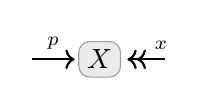
\begin{tikzpicture}[center base]
		\node[dpad0] (X) {$X$};
		\coordinate (A) at ($(X) + (-0.9,0)$);
		\draw[arr1] (A) -- node[above]{$\scriptstyle p$}  (X);
%
		\draw[arr2, <<-] (X) --  node[above,pos=0.8]{$\scriptstyle x$} ++(0.9, 0);
	\end{tikzpicture}
	}.
	\]
\end{linked}

In some ways, this result is entirely unsurprising, given that PDG scoring rule \eqref{eq:semantics} is a complicated and flexible formula built out of information theoretic primitives.
%
With a little more focus on the context and less on the algebra, perhaps \Cref{prop:pdg-Ix} becomes more curous: the inconsistency of the PDG containing just a distribution $p(X)$ and a sample $x$ just so happens to equal the overlwhelming favorite measure of incompatibility between a distribution $p$ and sample $x$ --- and it is known as ``surprise'', a particular kind of cognitive dissonance.
% Equation \eqref{eq:semantics} was not designed to do this.


A common justification for using $\I_p(x)$ as a cost for updating a probabilistic model $p(x)$ based on an observed sample $x$, is that by minimizing it, you  ``maximize the probability of seeing your data''.%
%
 	\footnote{this justification should not be taken too seriously  without constraints on $p$, because the optimal value of $p$  is $\delta_x$, which does not generalize.}
But this explanation applies just as well to $-p(x)$. Why include the logarithm?
There are plenty of answers to this question; among them: $\I_p$ is convex in $p$, it decomposes products into arguably simpler sums, is more numerically stable, has a well-defended physical analogue in thermodynamics, and is a primative of information theory.

For those after a quick and rigorous justification (as opposed to handwaving or a thermodynamics textbook), none of these answers are entirely satisfying.
They suggest that $\I_p$ has certain nice properties, but not that it enjoys them uniquely, or that no other loss function satisfies nicer ones.
Pedagogically speaking, the situation is more straightforward for us.
Although PDG semantics themselves require non-trivial justification (e.g., by direct appeal to information theory), they give us in return simple, intuitive, and uniform answers to many questions --- starting with following, simple one.
Why use the surprise $\I_p(x)$, to measure the loss of a model $p(X)$ on sample $x$? Because it is the inconsistency of simultanously believing $X = x$ and $x \sim p$.

For this argument to be pesuasive, one needs to accept our definition of inconsistency more broadly. \Cref{prop:pdg-Ix} is a very simple special case.
One concern is that it does not model the whole state of affairs; we train probabilstic models models with more than one sample.
What if we replce $x$ with an emperical distribution on many samples?
The first step in the proof of \cref{prop:pdg-Ix} is no longer valid, but we can get the same effect by being extremely confident in the data distribution.

\begin{linked}{prop}{many-equal-simple}
	Given a model determining a probability distribution with mass function $p(X)$, and samples $\xsamp = \{ x_i \}_{i=1}^m$ determining an emperical distribution $\datadist\xsamp$,  the following are equal, for all $\gamma \ge 0$:
	\begin{enumerate}
	\item The average negative log likelihood $\ell(p; \xsamp) = - \frac{1}{m} \sum_{i=1}^m \log p(x_i)$
	\item The cross entropy of $p$ relative to $\datadist\xsamp$
	\item $\bbr{\,p\,}_\gamma(\datadist\xsamp) ~{\color{gray}~+ (1+\gamma)\H(\datadist\xsamp)}$ \\[-1.4em]
	% FALSE! \item $\bbr{\,p^{\{\alpha=1\}} \,}_1 (\datadist\xsamp^{\{\alpha=1\}})$
	\item \(\aar[\Big] {
		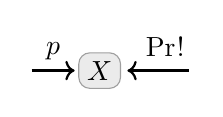
\begin{tikzpicture}[center base]
			\node[dpad0] (X) {$X$};
			\coordinate (A) at ($(X) + (-0.9,0)$);
			\draw[arr1] (A) -- node[above]{$p$}  (X);
			\draw[arr2, <-] (X) --  node[above,pos=0.6]{${\datadist\xsamp}!$} ++(1.2, 0);
				%\overset{\{\beta = \infty\}}
		\end{tikzpicture}
		}_\gamma
		~{\color{gray}~+ (1+\gamma) \H(\datadist\xsamp)}
		\)
	% \item
	% \(\aar[\Bigg] {
	% 	\begin{tikzpicture}[center base]
	% 		\node[dpad0] (X) {$X$};
	% 		\coordinate (A) at ($(X) + (-1.2,0)$);
	% 		\draw[arr1] (A) -- node[above,pos=0.4]{$ \overset {\{\alpha = 1\}} p$}  (X);
	% %
	% 		\draw[arr2, <-] (X) --  node[above,pos=0.6]{$ \overset{\{\beta = \infty,\alpha=\gamma\}}{\datadist\xsamp}$} ++(1.5, 0);
	% 	\end{tikzpicture}
	% 	}\!\bigg._1 \)
\end{enumerate}
\end{linked}

\begin{remark}
Note that the entropy of the data distribution $\H(\datadist\xsamp)$ does not depend on $p$, and so the final grey term in (3, 4) is not relevant for optimizing with respect to $p$.
\end{remark}

The PDG appearing in the final quantity of \cref{prop:many-equal-simple} is quite natural.
Aside from the certainty weights $\beta$, we've simply translated each piece of information into a cpd, and collected them together as a PDG.
We argue that the choice of $\beta$ makes sense as well, in the standard use cases for  cross entropy / log likelihood.
% In the current setting, we argue that the weights are also the ones we would expect.
The cross entropy measures the expected code length per sample, when a (possibly incorrect) distribution $p$ is used to design a code, in place of the true one $\datadist\xsamp$.
So implicitly, a modeler who chooses a cross-entropy has in some sense implicitly articulated a belief the data distribution is the ``true one'', by placing infinite certainty in $\datadist\xsamp$ than in $p$.
If $p(X)$ represents a probabilistic model before training is complete (say, a neural network with randomly initialized weights), we would be justified in placing dramatically more trust in the data $\datadist\xsamp$ than in $p$, and so this choice seems particularly appropriate.
% This justifies the `!'.
Other choices of $\beta$ are natural in other contexts, and we will see in \cref{sec:statdist} that they correspond to other losses. (For instance when $\beta_p = \beta_{\datadist\xsamp} = \nicefrac12$, the result is the Bhattacharyya distance, rather than the cross entropy.)


We now consider an orthogonal generalization of \cref{prop:pdg-Ix}, in which $x$ is only a partial observation of a joint model of two variables $X,Z$. In this case, we might hope to recover the \emph{marginal} negative log likelihood, since $Z$ does not interact with the observation. % ---  in \cref{prop:marginal-ll}.

\begin{linked}{prop}{marginal-ll}
	If $p(X,Z)$ is a joint distribution, the information content of the partial observation $X=x$, or the marginal negative log likelihood of $x$, is given by
	\begin{equation}
	 	\I_p(x) = \log \frac{1}{p(x)} =
	    % \lim_{t \to \infty}
		 \aar[\Bigg]{
	% 	  \Inc\left(
			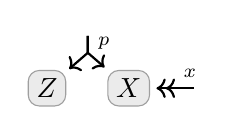
\begin{tikzpicture}[center base]
				\node[dpad0] (Z) {$Z$};
				\node[dpad0,right=.5 of Z] (X) {$X$};
				\coordinate (A) at ($ (X)!.5!(Z) + (0,0.7)$);
				\draw[arr1] (A) -- node[right]{$\scriptstyle p$} ++(0,-0.25) -- (X);
				\draw[arr1] (A) -- ++(0,-0.25) -- (Z);
	%
				\draw[arr2, <<-] (X) --  node[above,pos=0.8]{$\scriptstyle x$} ++(0.9, 0);
	% 			\draw[arr2, <-] (Z) -- node[above,pos=0.6]{$\scriptstyle q^{\{\beta =\infty\}}$} ++(-0.9, 0);%
				% \ar[r,"p"] \& Z \ar[r,"p", bend left] \& X \ar[l,"q", bend left] \& \ar[l, two heads, "x"']
			\end{tikzpicture}
			}.
			\label{eq:mll}
	\end{equation}
\end{linked}

Intuitively, the inconsistency in the PDG on the right hand side of \eqref{eq:mll} is localized to $x$, where the sample conflicts with the distribution; other variables don't make a difference.

% Furthermore, $p$ is the qualitative model we have in mind, and so we set $\alpha_p = 1$
In much the same way as \cref{prop:many-equal-simple} generalizes \cref{prop:pdg-Ix} by considering more than one sample at once, we also can obtain a multi-sample analogue of analog of \Cref{prop:marginal-ll}.

\begin{linked}{prop}{pdg-loglikelihood}
	The average negative log likelihood $\ell(p;x) := -\frac{1}{|\xsamp|}\sum_{x \in \xsamp} \log p(x)$ (which is also the cross entropy) is the inconsistency of the PDG containing $p$ and the data distribution $\datadist\xsamp$, plus the entropy of the data distribution (which is constant in $p$).
	That is,
	\[
	\ell(p;\xsamp) =
	 \aar[\Bigg]{
	 % \Inc\left(
		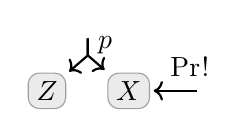
\begin{tikzpicture}[center base]
			\node[dpad0] (Z) {$Z$};
			\node[dpad0,right=.5 of Z] (X) {$X$};
			\coordinate (A) at ($ (X)!.5!(Z) + (0,0.7)$);
			\draw[arr1] (A) -- node[right]{$p$} ++(0,-0.25) -- (X);
			\draw[arr1] (A) -- ++(0,-0.25) -- (Z);
			%
			\draw[arr1, <-] (X) --  node[above,pos=0.8]{$\datadist\xsamp!$} ++(0.9, 0);
			% \draw[arr1, <-] (Z) -- node[above]{$\scriptstyle q$} ++(-0.9, 0);
		\end{tikzpicture}
		}%_{\!\!0}
		% \right)
		+ \H(\datadist\xsamp).
	\]
\end{linked}


So far we have been considering models of a distribution $p(X)$ that correspond to generative models, or an unsupervised setting. In the supervised setting, in which our model predicts $Y$ from $X$, and is trained from joint samples ($X,Y$), cross entropy loss is perhaps even more dominant. And it equals the inconsistency of a PDG consisting of the predictor $f(Y|X)$ together with high-confidence data.

\begin{linked}{prop}{supervised-cross-entropy}
	Consider a probabilistic model $f$ with mass function $f(y\mid x)$. The inconsistency of the PDG containing $p(y \mid x)$ and the emperical distribution $\datadist\xysamp$ of samples $\xysamp$ is equal to the negative log-liklihood (cross-entropy) loss, plus the emperical uncertainty in $Y$ given $X$ (a constant independent of $f$). That is,
	\[ \aar**{
		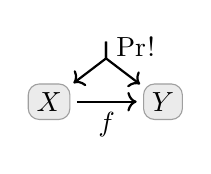
\begin{tikzpicture}[center base]
			\node[dpad0] (Y) {$Y$};
			\node[dpad0,left=.9 of Y] (X) {$X$};
			\coordinate (A) at ($ (X)!.5!(Y) + (0,0.8)$);
			\draw[arr1] (A) -- node[right]{$\datadist\xysamp!$} ++(0,-0.25) -- (X);
			\draw[arr1] (A) -- ++(0,-0.25) -- (Y);
			\draw[arr2, ->] (X) --  node[below,pos=0.5]{$f$} (Y);
		\end{tikzpicture}} = \frac1{|\xysamp|}\sum_{(x,y) \in \xysamp} \left[ \log \frac1{f(y \mid x)}\right] \quad - \H_{\datadist\xysamp}(Y\mid X).
	\]
\end{linked}

\begin{remark} \label{remark:continuous}
\cref{prop:pdg-Ix,prop:many-equal-simple,prop:marginal-ll,prop:pdg-loglikelihood,prop:supervised-cross-entropy} all require the probability to have a mass function, rather than a density function, which implicitly restricts us to discrete variables.
A PDG containing both a continuous distribution function and a discrete empmerical distribution is infinitely consistent, because the probability of any particular sample is zero.
Indeed, the analog of surprise $-\log p(X)$ is not well-founded for a density $p(X)$, because $p(X)$ is not dimensionless, but rather in inverse $X$-units, so depends on an (arbitrary) choice of scale.
However, such a rescaling only amounts to adding a constant.

Furthermore approximating $p(X)$ with a discretization also only contributes a constant, in the sense that the analogues of \cref{prop:pdg-Ix,prop:many-equal-simple,prop:marginal-ll,prop:pdg-loglikelihood,prop:supervised-cross-entropy} in which a density function is used in place of a mass function, are identical--- save for an additive constant depending only discretization size.
But this additive constant is irrelevant for optimization,
and so in this sense the results here also justify use of the continuous analogues (such as $- \log p(X)$ for a pdf $p$) as loss functions, even though these functions are not invariant with respect to changes of parameterization.
\end{remark}

\subsection{Simple Performance Metrics as Inconsistencies}

There are also simpler scoring metrics used to evaluate the performance of systems on datasets, such as the accuracy of a  classifier, or the mean-squared error of a regressor?

\begin{linked}[log accuracy as inconsistency]
		{prop}{accuracy}
	If $h: X \to Y$ is a predictor for an input space $X$ and label space $Y$, and $f: X \to Y$ generates the correct labels, then the inconsistency of believing $f$ and $h$ (with any degree of confidence), and also that inputs are distributed according to $D(X)$, equals the information content of learning that $f(X) = h(X)$ according to $D$ (which is the log accuracy of the predictor $h$) times the confidence in $D$. That is,
	\begin{equation}\label{eq:accuracy-pdg}
		\aar*{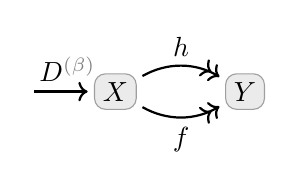
\begin{tikzpicture}[center base]
				\node[dpad0] (Y) {$Y$};
				\node[dpad0,left=1.1 of Y] (X) {$X$};
				%
				\draw[arr2, ->>] (X) to[bend left] node[pos=0.5, above]{$h$} (Y);
				\draw[arr2, ->>] (X) to[bend right] node[pos=0.5, below]{$f$} (Y);
				\draw[arr2, <-] (X) to node[pos=0.4, anchor=south west, above]
					% {$\overset{(\beta)}D$} +(-1.1, 0);
					{$D^{\color{gray}(\beta)}$} +(-1.1, 0);
			\end{tikzpicture}}
		=  - \beta\,\log \Big( \mathrm{accuracy}_{f,D} (h) \Big)
		= \beta\, \I_D [f = h].
	\end{equation}
\end{linked}
It is common to think of accuracy as a property of a hypothesis $h$ (with some dependence on the true labeling function $f$ and the data distribution $D$), even though it is symmetric in $f$ and $g$, in part because we change the predictor more than the labels.
The correspondence of \Cref{prop:accuracy} graphically depicts this symmmetry, and also a more subtle phenomenon: a particularly strong dependence on the distribution of inputs.
In fact, the inconsistency of the PDG in \eqref{eq:accuracy-pdg} is scaled by the confidence of $D$, but does not depend at all on the confidences in $h$ or $f$.

% TODO: Why should this be the case?
Why should this be the case? The deterministic nature of $f$ and $h$ encodes extreme confidence (to anthropomorphise: $f$ thinks it impossible that $Y \ne f(X)$, because that event has probability zero), and so the only way to selectively choose samples to make things consistent is to alter the distribution of \emph{inputs} $\Pr(X)$ (so that it is always the case that $f(x) = g(x)$), not to change $\Pr(Y \mid X)$.
But it is the direction that we want to pull $\Pr(Y\mid X)$ that informs how we should update our predictor $h(Y \mid X)$, which reflects the non-differentiability of the accuracy (or zero-one loss) with respect to $h$.
Note that this is a the complete opposite of how we captured cross entropy (\cref{prop:supervised-cross-entropy}), in which we are unwilling to budge on the data distribution, but are willing to modify our predictor $h$.


%Confusion matrix costs
% \begin{prop}
% 	\[
% 	\]
% \end{prop}


When $Y$ is a continuous variable rather than a discrete one, the estimator is referred to as a regressor, rather than a classifier, and the topology of the real numbers comes with an intuition that not all mistakes are equally bad; a small deviation from the correct value of $Y$ is close to correct.
Perhaps the most common way of measuring this deviation is with mean square error, which corresponds to the inconsistency of believing that $f$ and $h$ control the mean of a unit-variance gaussian.
But before we get there, we first prove a more general result, which is most clearly articulated in terms of a power mean.

\begin{defn}%[power mean]
	The weighted power mean $\mathrm M^w_p(\mathbf r)$ of the collection of real numbers $\mathbf r = r_1, \ldots, r_n$ with respect to the convex weights $w = w_1, \ldots, w_n$ satisfying $\sum_iw_i = 1$, is given by
	\[ \mathrm M^w_p(\mathbf r) := \Big(\sum_{i=1}^n w_i (r_i)^p \Big)^{\frac1p}.\]
	We omit the superscript as a shorthand for the uniform weighting $w_i = \nicefrac{1}{N}$.
	Most standard means, such as those in \cref{tab:power-means}, are special cases.
\end{defn}

\begin{table}
\centering
\renewcommand{\arraystretch}{1.5} % General space between rows (1 standard)
\begin{tabular}{rcl}
	\textbf{Name} & $p$ & \textbf{Formula}\\\hline
	Harmonic&$(p=-1)$:& $\mathrm{HM}_w(\mathbf r) = \faktor1{\left(\sum_{i=1}^n \nicefrac{w_i}{r_i}\right)}$ \\
	Geometric&$(\lim {p\to 0})$:& $\mathrm{GM}_w(\mathbf r) = \prod_{i=1}^n r_i^{w_i}$ \\
	Arithmetic&$(p=1)$:& $\mathrm{AM}_w(\mathbf r) = \sum_{i=1}^n w_i r_i$ \\
	Quadratic&$(p=2)$:& $\mathrm{QM}_w(\mathbf r) = \sqrt{\textstyle\sum_{i=1}^n w_i r_i^2}$\\\hline
	\end{tabular}
	\caption{special cases of the $p$-power mean $\mathrm M_p^w(\mathbf r)$}
	\label{tab:power-means}
\end{table}
% \begin{align*}
% 	\text{Harmonic}~(p=-1):&\quad \mathrm{HM}_w(\mathbf r) = \frac1{\sum_{i=1}^n \nicefrac{w_i}{r_i}} \\
% 	\text{Geometric}~(\lim {p\to 0}):&\quad \mathrm{GM}_w(\mathbf r) = \prod_{i=1}^n r_i^{(w_i)} \\
% 	\text{Arithmetic}~(p=1):&\quad \mathrm{AM}_w(\mathbf r) = \sum_{i=1}^n w_i r_i \\
% 	\text{Quadratic}~(p=2):&\quad \mathrm{QM}_w(\mathbf r) = \sqrt{\textstyle\sum_{i=1}^n w_i r_i^2}.
% \end{align*}

It is well known that $\mathrm M_p^w(\mathbf r)$ is increasing in $p$, and strictly so if not all elements of $\mathbf r$ are identical. In particular, $\mathrm{QM}_w(a,b) > \mathrm{GM}_w(a,b)$ for all $a \ne b$ and positive weights $w$. We now present the result.


\begin{linked}{prop}{inc-two-gaussians}
	Consider a PDG containing two (distinct) conditional Gaussian distributions on a variable $Y$, whose parameters can both depend on a variable $X$. Its inconsistency takes the form
	\begin{align*}
		\aar**{\!\!\!\!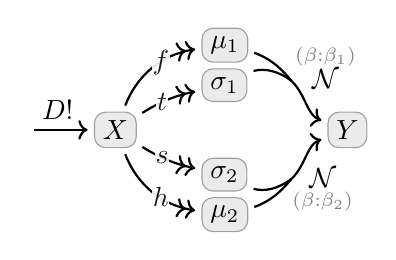
\begin{tikzpicture}[center base]
			\node[dpad0] (Y) {$Y$};
			\node[dpad0,left=2.4 of Y] (X) {$X$};
			\node[dpad0,above right=0.6 and 0.8 of X] (mf) {$\mu_1$};
			\node[dpad0,below right=0.6 and 0.8 of X] (mh) {$\mu_2$};
			\node[dpad0,above right=0.1 and 0.8 of X] (sf) {$\sigma_1$};
			\node[dpad0,below right=0.1 and 0.8 of X] (sh) {$\sigma_2$};
			%
			\draw[arr2, ->>] (X) to[bend left=30]
				node[pos=0.6, inner sep=0.2pt, fill=white, fill opacity=0.9] {$f$} (mf);
				\draw[arr2, ->>] (X) to[bend left=10]
					node[pos=0.4, inner sep=0.2pt, fill=white, fill opacity=0.9] {$t$} (sf);
			\draw[arr2, ->>] (X) to[bend right=30]
					node[pos=0.6, inner sep=0.2pt, fill=white, fill opacity=0.9] {$h$} (mh);
				\draw[arr2, ->>] (X) to[bend right=10]
					node[pos=0.4, inner sep=0.2pt, fill=white, fill opacity=0.9] {$s$} (sh);
			%
			\draw[arr2, <-] (X) to node[pos=0.55, above]{$D!$} +(-1.1, 0);
			\coordinate (C1) at ($(mf)!.5!(sf) + (0.85,-0.2)$);
			\coordinate (C2) at ($(mh)!.5!(sh) + (0.85,+0.2)$);
			% \coordinate (C2) at ($ (X)!.5!(Y) + (0,0.8)$);
			\draw[arr2, ->] (mh) to[bend right=15] (C2) to[out=45,in=-160]
				node[pos=0.25, below right, inner sep=0] {\!\!$\underset{{\color{gray}(\beta:\beta_2)}}{\mathcal N}$} (Y);
			\draw[arr2, -,shorten >=0pt] (sh) to[bend right=25] (C2);
			%
			\draw[arr2, ->] (mf) to[bend left=15] (C1) to[out=-45,in=160]
				node[pos=0.25, above right, inner sep=1pt] {\!\!$\overset{{\color{gray}(\beta:\beta_1)}}{\mathcal N}$} (Y);
			\draw[arr2, -,shorten >=0pt] (sf) to[bend left=25] (C1);
			% \draw (current bounding box.north east) rectangle (current bounding box.south west);
		\end{tikzpicture}\!} %\hspace{-2cm}&\\
		 \! &=
		  	\frac12
			\Ex\nolimits_D \!\!\left[
		 	{\mathrm {HM}}(\beta_1, \beta_2)
				\frac12
			\left( \frac{\mu_1 - \mu_2}
		 		{\mathrm {QM}_{\hat\beta}(\sigma_1,\sigma_2)} \right)^{\!\!2}
			+ {\mathrm {AM}}(\beta_1, \beta_2) \log
				\frac
				{\mathrm {QM}_{\hat\beta}(\sigma_1,\sigma_2)}
				{\mathrm {GM}_{\hat\beta}(\sigma_1,\sigma_2)}
		 \right] \numberthis\label{eq:2gaussians} \\
		 &\color{gray}\hspace{-2cm}= \Ex_{x \sim D} \left[
		 	\frac{\beta_1 \beta_2}2
		 	\frac{\Big(f(x) - h(x)\Big)^2}
		 		% {\mathrm {QM}_{\hat\beta}(s(x),t(x))}
		 		{\beta_2 s(x)^2 + \beta_1 t(x)^2}
			+ \frac{\beta_1 + \beta_2}{2} \log
				\frac
				{\beta_2 s(x)^2 + \beta_1 t(x)^2}
				{(\beta_1 + \beta_2)( s(x)^{\beta_2} t(x)^{\beta_1})^{\frac1{\beta_1+\beta_2}}}
				% {\mathrm {QM}_{\hat\beta}(s(x),t(x))}
				% {\mathrm {GM}_{\hat\beta}(s(x),t(x))}
		 \right]
	\end{align*}
	where  $\hat\beta = (\frac{\beta_2}{\beta_1+\beta_2}, \frac{\beta_1}{\beta_1+\beta_2})$ represents the normalized and reversed vector of conficences $\beta = (\beta_1, \beta_2)$ for the two distributions, and $\mu_1 = f(X)$, $\mu_2 = g(X)$, $\sigma_1 = s(X)$, $\sigma_2 = t(X)$ are random variables over $X$.
\end{linked}


Plugging in $s(x) = t(x) = 1$ and $\beta_1 = \beta_2 = 1$ gives us the result we had hinted at before.

\begin{coro}[Mean Square Error as inconsistency] \label{coro:MSE}
	\begin{align*}
		\aar**{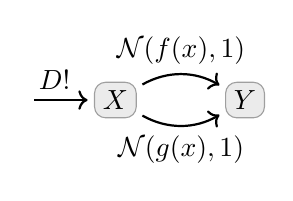
\begin{tikzpicture}[center base]
			\node[dpad0] (Y) {$Y$};
			\node[dpad0,left=1.1 of Y] (X) {$X$};
			%
			\draw[arr2, ->] (X) to[bend left]
				node[pos=0.5, above] {$\mathcal N(f(x), 1)$} (Y);
			\draw[arr2, ->] (X) to[bend right] node[pos=0.5, below]{$\mathcal N(g(x), 1)$} (Y);
			\draw[arr2, <-] (X) to node[pos=0.6, above]{$D!$} +(-1.1, 0);
		\end{tikzpicture}}
		&=
		\aar**{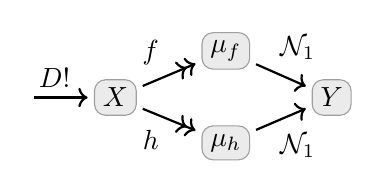
\begin{tikzpicture}[center base]
			\node[dpad0] (Y) {$Y$};
			\node[dpad0,left=2.2 of Y] (X) {$X$};
			\node[dpad0,above right=0.1 and 0.8 of X] (mf) {$\mu_f$};
			\node[dpad0,below right=0.1 and 0.8 of X] (mh) {$\mu_h$};
			%
			\draw[arr2, ->>] (X) to[bend left=0]
				node[pos=0.5, above left=0] {$f$} (mf);
			\draw[arr2, ->>] (X) to[bend right=0]
				node[pos=0.5, below left=0] {$h$} (mh);
			%
			\draw[arr2, <-] (X) to node[pos=0.6, above]{$D!$} +(-1.1, 0);
			%
			\draw[arr2, ->] (mh) to[bend right=0]
				node[pos=0.3, below right=0] {$\mathcal N_1$} (Y);
			\draw[arr2, ->] (mf) to[bend left=0]
				node[pos=0.3, above right=0]{$\mathcal N_1$} (Y);
			% \draw[arr2, <-] (X) to node[pos=0.6, above]{$D$} +(-1.1, 0);
		\end{tikzpicture}}\\
		 &= \Ex\nolimits_D \Big( f(X) - h(X) \Big)^2
		 =: \mathrm{MSE}( f, h ), \numberthis\label{eq:mse}
	\end{align*}
	where $\mathcal N_1 = \mathcal N(-,1)$ is the normal distribution with unit variance, and mean equal to its argument.
\end{coro}

The equality of the two PDG inconsistencies illustrates an orthogonal point: that PDGs handle composition of functions as one would expect, so that it is equivalent to model an entire process as a single arrow, or to break it into stages, ascribing an arrow to each stage, with one step of randomization.




%%%%%%%%%%%%%%%%%%%%%%%%%%%%%%%%%%%%%%%%%%
% The fact that $\mathrm{QM}(a, b) > \mathrm{GM}(a,b)$ for $a, b >0$ has been used to movivate a metric  between different power means is sometimes used to measure the
% \eqref{eq:2gaussians} and  gives
% \begin{equation*}
% \aar**{\begin{tikzpicture}[center base]
% 	\node[dpad0] (Y) {$Y$};
% 	%
% 	% \draw[arr2, ->] (X) to[bend left]
% 	% 	node[pos=0.5, above] {$\mathcal N(0, s(x))$} (Y);
% 	% \draw[arr2, ->] (X) to[bend right] node[pos=0.5, below]{$\mathcal N(0, t(x))$} (Y);
% 	\draw[arr2, <-] (Y) to node[pos=0.6, above]{$\mathcal N(0, \sigma_1)$} +(-1.4, 0);
% 	\draw[arr2, <-] (Y) to node[pos=0.6, above]{$\mathcal N(0, \sigma_2)$} +(1.4, 0);
% \end{tikzpicture}}
% =  \log
% 	 \frac
% 	 {\mathrm {QM}(\sigma_1,\sigma_2)}
% 	 {\mathrm {GM}(\sigma_1,\sigma_2)}
% \end{equation*}




% % The results in this section may not teach us very much that we did not know before, but
% Although the results in this section are not particularly useful on their own,
% they do display at a surprisingly strong tie between the standard metrics used to train probabilistic models, and the inconsistency of a corresponding PDG ---
% we have seen that (marginal) log likelihood, cross entropy, and log accuracy all arise naturally as inconsistencies of the appropriate PDGs.


%%%%%%%%%%%%%%%%%%%%%%%%%%%%%%%%%%%%%%%%%%%%%%%%%%%/%%%%%%%%%%%%%%%%%%%%%%
\section{Statistical Distances as Inconsistencies} \label{sec:statdist}
Suppose you are concerned with only a single variable $X$. One friend has told you that it is distributed according to the probability distribution $p(X)$; another has told you that it follows $q(X)$. You adopt both beliefs. If $p \ne q$, your mental state will be inconsistent, and more so the more $p$ and $q$ differ.
As a result, we can view of the inconsistency of a PDG containing only a single varible $X$ and two distributions $p(X)$ and $q(X)$ over it, as a measure of divergence.

Recall that a PDG also allows us to specify the confidences $\beta_p$ and $\beta_q$ of each edge, and so we can form a distinct PDG containing only the distributions $p$ and $q$ for each setting of $(\beta_p, \beta_q)$.
It turns out that a surprisingly large classs of statistical distances arise as the inconsistency of such a PDG.
We start with the case in which one confidence becomes arbitrary large.

\begin{prop}[KL Divergence as Inconsistency]
	The inconsistency of believing $p$ with complete certainty, and also $q$ with some finite certainty $\beta$, is $\beta$ times the KL Divergence (or relative entropy) of $q$ with respect to $p$. That is,
\[
    \aar[\bigg]{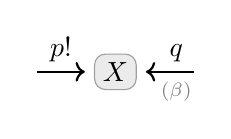
\begin{tikzpicture}[center base]
        \node[dpad0] (X) {$X$};
        \draw[arr, <-] (X) -- node[above]
            {$p !$}  ++(-1.1,0);
        \draw[arr, <-] (X) --  node[above,pos=0.6]
            % {$\overset{\smash{\color{gray}(\beta)}}q$} ++(0.9, 0);
         	% {$\overset{{\color{gray}(\beta)}}q$}
            % {$q~^{{\color{gray}(\beta)}}$} ++(1.1, 0);
			{$q$}
			node[below,pos=0.6]{$\scriptstyle{\color{gray}(\beta)}$}++(1.1, 0);
    \end{tikzpicture}}
	= \beta\, \kldiv pq
\]
\end{prop}
This result gives us an intuitive interpretation of the asymmetry of relative entropy / KL divergence, and a prescription about when it makes sense to use it.
$\kldiv p q$ is the inconsistency of a mental state containing both $p$ and $q$, when absolutely certain of $p$ (and not willing to budge on it).
This concords with the standard view that $\kldiv pq$ reflects the amount of information required to change $q$ into $p$, which is why we call it the relative entropy ``from $q$ to $p$''.


In general, we derive the following form for the inconsistency of a PDG whose contents are distributions $p(X)$ and $q(X)$, for arbitrary confidences.
\begin{linked}{lemma}{pdgdiv}
	The PDG divergence $\thickD^{\mathrm{PDG}}_{(r,s)}(p, q)$, the inconsistency of a PDG containing $p(X)$ with confidence $r$ and $q(X)$ with confidence $s$, satisfies
    \[
		\thickD^{\mathrm{PDG}}_{(r,s)}(p, q) :=
        \aar[\bigg]{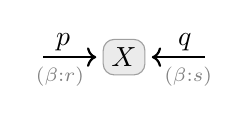
\begin{tikzpicture}[center base]
            \node[dpad0] (X) {$X$};
            \draw[arr2, <-] (X) --
			 		% node[above] {$\overset{(\beta : r)}p$}
			 		node[above, pos=0.6, inner sep=2pt, align=center] {$p$}
			 		node[below, pos=0.65, inner sep=3pt, align=center] {$\scriptstyle{\color{gray}(\beta : r)}$}
				++(-1.1,0);
            \draw[arr2, <-] (X) --
					% node[above,pos=0.5] {$\overset{(\beta : s)}q$}
			 		node[above, pos=0.6, inner sep=2pt, align=center] {$q$}
			 		node[below, pos=0.65, inner sep=3pt, align=center] {$\scriptstyle{\color{gray}(\beta : s)}$}
				 ++(1.1, 0);
        \end{tikzpicture}}
        % = \thickD^{\mathrm{PDG}}_{(r,s)}(p, q)
        = - (r+s) \log  \sum_x \left(p(x)^{r}\vphantom{\Big|} q(x)^{s}\right)^{\frac{1}{r+s}}.
        % = - (r+s) \log \sum_x \! \sqrt[\leftroot{0}\uproot{2}r+s]{\vphantom{\big|}p(x)^{r} q(x)^{s}}
    % \qquad\text{where}\qquad \xi:= \beta_p+\beta_q
    \]
\end{linked}


\begin{figure}
	\centering
	\def\ptradius{0.07}
	\begin{tikzpicture}[scale=1.8]
		\draw[help lines, color=gray!30, dashed] (-0.9,-1.4) grid (5.9,2.9);
		\draw[->,thick] (-1,0)--(6,0) node[right]{$\beta_p$};
		\draw[->,thick] (0,-1.5)--(0,3) node[above]{$\beta_q$} ;


		%concave part
		\fill[gray, fill opacity=0.2] (-1,1) -- (1.5,-1.5) -- (-1,-1.5) --cycle;
		\draw[gray, opacity=0.5, thick] (-1,1) --
		node[below left=3em, anchor=north, rotate=-45,font=\footnotesize,fill=gray!20,fill opacity=0.8, inner sep=1pt, outer sep=3pt] % at (-0.5,-0.5)
			{Non-convex region} (1.5,-1.5);
		%axis of symmetry
		% \draw[color=orange!25, thick] (-1, -1) -- (3,3);
		% \fill[orange, opacity=0.05] (-1,-1) -- (3,3) -- (-1,3) -- cycle;
		\draw[color=gray!80!orange!45, densely dashdotted] (-1, -1) -- (3,3);
		\draw[color=gray!80!orange!45, thick, <->] (2.8, 2.2) -- node[above right, anchor=south, rotate=-45,font=\footnotesize,fill=white,fill opacity=0.8, inner sep=1pt, outer sep=3pt]{Axis of Symmtry}(2.2,2.8);


		% Renyi Entropy Line
		\draw[blue!40, densely dashed, very thick, opacity=0.8]
		 	(0,1) -- node[below, align=center, pos=0.8, font=\footnotesize]{R\'enyi divergences\\for $\alpha \in (0,1)$} (5.6,1)
			(5.6,-1) -- node[above, align=center, pos=0.2, font=\footnotesize]{(negative) R\'enyi divergences\\ for $\alpha \in (1,\infty)$} (1,-1);
		%Chernoff Information Line
		\draw[red, densely dashed, very thick, opacity=0.9, (-), shorten <=6pt, shorten >=6pt]
		 	(0,1) -- node[pos=0.5,below left=5pt,anchor=north, rotate=-45, font=\footnotesize, align=center, fill=white,fill opacity=0.8, inner sep=1pt, outer sep=3pt]{Chernoff\\Divergences} (1,0);
		%alpha divergence line
		\draw[domain=1.5:5.6, smooth, very thick, variable=\x, blue!50!green!50, opacity=0.8, densely dashed] plot ({\x}, {1/(1-1/\x)})
			node[rotate=-7, font=\footnotesize] at (3.9,1.55){$\alpha$-divergences};

		%%%% POINTS %%%%
		%[draw, very thick,fill=magenta!50!black]
		\fill (0.5,0.5) circle (\ptradius) node[above right, align=center,
			label={[yshift=0ex,xshift=-1ex,align=left,font=\footnotesize\color{gray!50}]right:Bhattacharya\\distance}]
			% {Bhattacharya\\distance};
			% {$\thickD^{\text{Bhattacharya}}$};
			{$\thickD_{B}(p,q)$};

		\fill (1,3.4) -- +(0:\ptradius) arc (0:-180:\ptradius) -- +(0:\ptradius)
			node[below]{$\vdots$}
			node[right=1ex, align=center,label={[yshift=1ex,xshift=0ex]below:\footnotesize\color{gray!50}Reverse KL}](revKL){$\kldiv qp$};

		\fill (6.4,1) -- +(270:\ptradius) arc (270:90:\ptradius) -- +(270:\ptradius)
			node[above=2pt, align=center,
				label={[yshift=-1ex,xshift=0ex]\footnotesize\color{gray!50} KL Divergence}] (FwdKL) {$\kldiv pq$}
			node[left]{$\cdots$};

		\fill (0,1) -- ++(-90:\ptradius) arc (-90:90:\ptradius)
			node[above right, align=center,
				label={[yshift=-1ex,xshift=1ex]\footnotesize\color{gray!50} Max Entropy}
			]{$\I_q(p > 0)$};

		% divergences requiring negative \beta
		\fill (2,-1) circle (\ptradius) node[below right, align=center,
				label={[yshift=1ex,xshift=1ex]below:\footnotesize\color{gray!50}$-\chi^2$ divergence}]
			{$-\chi^2\infdivx pq$};
		\fill (1,-1) -- ++(-45:\ptradius) arc (-45:135:\ptradius)
			node[above, align=center,
				label={[yshift=-1ex,xshift=1ex]\footnotesize\color{gray!50} $-$Min Entropy}]
			{$- \log \sup \frac pq$};



	\end{tikzpicture}
	\caption{A map of the inconsistency of the PDG containing the distributions $p(X)$ and $q(X)$, as we vary their respective confidences $\beta_p$ and $\beta_q$. Solid circles indicate well-known named measures, and semicircles indicate limiting values. }
	% {A map of inconsistency
	% \(\aar[\bigg]{\begin{tikzpicture}[center base]
	% 	\node[dpad0] (X) {$X$};
	% 	\draw[arr2, <-] (X) --
	% 			node[above, pos=0.6, inner sep=2pt, align=center] {$p$}
	% 			node[below, pos=0.65, inner sep=3pt, align=center] {$\scriptstyle{\color{gray}(\beta_p)}$}
	% 		++(-1.1,0);
	% 	\draw[arr2, <-] (X) --
	% 			node[above, pos=0.6, inner sep=2pt, align=center] {$q$}
	% 			node[below, pos=0.65, inner sep=3pt, align=center] {$\scriptstyle{\color{gray}(\beta_q)}$}
	% 		 ++(1.1, 0);
	% \end{tikzpicture}}\)
	% as we vary the confidences $(\beta_p, \beta_q)$ in the distributions $p$ and $q$. }
	\label{fig:statdistmap}
\end{figure}




Of the many generalizations of KL divergence, R\'enyi divergences, first characterized by Alfr\'ed R\'enyi \cite{renyi1961measures} are perhaps the most significant, as few others have found either application or an interpretation in terms of coding theory \cite{van2014renyi}.
The R\'enyi divergence of order $\alpha$ between two distributions $p(X)$ and $q(X)$ is given by
\begin{equation}
	\thickD_\alpha\infdivx p q := \frac{1}{1- \alpha} \sum_{x \in \V(X)} p(x)^\alpha q(x)^{1-\alpha}\label{eq:renyi}
\end{equation}
R\'enyi introduced this measure in the same paper as the more general class of $f$-divergences, but directs his attention towards those of the form \eqref{eq:renyi}, because satisfy a natural weakening of Fadeev's postulates \cite{fadeev1957begriff}, for Shannon entropy.
Concretely, every symmetric, continuous measure that additively separates over independent events, and with a certain `mean-value property', is of the form \eqref{eq:renyi}, up to scaling \cite{renyi1961measures}.
It follows from \cref{lemma:pdgdiv} that varing the confidences of our two-distribution PDG, essentially carves out the same class: every R\'enyi entropy is the inconsistency of some PDG of this form, and every PDG divergence (with the exception of limiting values) is a scaled R\'enyi entropy.

\begin{coro}[R\'enyi Divergences as Inconsistencies]
    \[ \thickD^{\mathrm{PDG}}_{r, s}(p, q) =
        s \cdot \thickD_{\frac{r}{r+s}}\infdivx{p}{q}
    \qquad \text{and} \qquad
        \thickD_{\alpha}\infdivx{p}{q}
        = \thickD^{\mathrm{PDG}}_{\left(\frac{\alpha}{1-\alpha}, 1\right)}(p, q).
    \]
\end{coro}

However, the two classes are not exactly identical, because the PDG divergences admit extra limit points. One of the biggest differences is that the reverse KL divergence $\kldiv q p$ is not a Renyi entropy of the form $\thickD_\alpha\infdivx p q$ for any value (or limit) of $\alpha$. This lack of symmetry has caused other authors to instead work with a re-scaled symmetric version of the R\'enyi entropy, called $\alpha$-divergence  \cite{cichocki2010families} (although sometimes the term is used for the same quantity without the logarithm).  The relationship between them can be seen in \cref{fig:statdistmap}.


We submit that viewing these as inconsistencies can clarify things a great deal. Whereas the formula for R\'enyi entropy is mostly symmetric, the leading $\frac1\alpha$ makes it instead \emph{skew}-symmetric, and does not directly reduce to reverse KL divergence. PDG ``divergences'', on the other hand, are symmetric: the semantics do not give special treatment to one edge over the other.

One consequence of representing divergences as inconsistencies is that we can use \cref{lemma!} to derive relationships between them. The following facts follow immediately, and can be seen in \cref{fig:statdistmap} by inspection.
\begin{coro}
	\begin{enumerate}[nosep]
		\item R\'enyi entropy is monotonic in its parameter $\beta$
		\item $\kldiv P Q \ge 2 \thickD_B(P,Q) \le \kldiv Q P$
		\item If $Q(P > 0) < 1$ (i.e., $Q \not\ll P$), then $\kldiv Q P = \infty$
	\end{enumerate}
\end{coro}

The Chernoff divergence, used in Bayesian hypotehsis testing, measures the tightest possible exopnent to bound the probability of error \cite{nielsen2011chernoff}. It also happens to be the smallest possible inconsistency of simultaneously believing $p$ and $q$, with combined confidence 1.
\begin{coro}[Chernoff Divergence as Inconsistency]
\[
	\inf_{\beta \in (0,1)}
	\aar[\bigg]{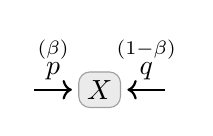
\begin{tikzpicture}[center base]
		\node[dpad0] (X) {$X$};
		\draw[arr2, <-] (X) -- node[above]
			{$\overset{(\beta)}p$}  ++(-0.9,0);
		\draw[arr2, <-] (X) --  node[above,pos=0.5]
			{$\overset{(1-\beta)}q$} ++(0.9, 0);
	\end{tikzpicture}}
	% = \thickD^{\mathrm{PDG}}_{(r,s)}(p, q)
	= \thickD^{\text{Chernoff}}(p,q)
	% = - (r+s) \log \sum_x \! \sqrt[\leftroot{0}\uproot{2}r+s]{\vphantom{\big|}p(x)^{r} q(x)^{s}}
% \qquad\text{where}\qquad \xi:= \beta_p+\beta_q
\]
\end{coro}

All of these results are only for simple PDGs, containing one variable and two distributions.
Inconsistency of general PDGs, then is in some sense a vast generalization of the Renyi divergences to structured objects.

\section{Regularizers and Priors}
\label{sec:regularizers}
The picture presented here is compatible with the correspondence between regularization and Bayesian priors; as has been noted by other authors \cite{williams1995bayesian,rennie2003l2,probinterpblogpost,mitcourse}, L2 regularization corresponds to a Gaussian prior \cite{rennie2003l2}, and indeed adding such a distribution to the PDG gives an extra term in the consistency, equal to the L2 regularizer. Similarly, the L1 regularizer corresponds to a Leplacian prior \cite{williams1995bayesian}.

We now review these findings in the context of our framework, as we show how adding a prior distribution in a PDG results in the corresponding regularization term in the inconsistency.

\begin{linked}{prop}{regularized}
	Consider a situation where you believe that $Y$ is distributed according to $f_\theta(Y)$  for some parameter $\theta$, and also that you have a prior belief $p(\theta)$ over parameters, and an emperical distribution $D$ over $Y$ which you trust. The inconsistency of also believing that the parameter is some $\theta_0$ is the \emph{regularized}-cross entropy loss, where the regularizer is $\log \frac1{p(\theta_0)}$ times the confidence in the prior $p$.
	That is,
	\begin{equation}\label{eq:regularize}
		\aar*{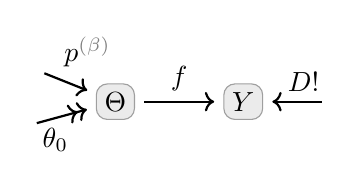
\begin{tikzpicture}[center base]
			\node[dpad0] (theta) {$\Theta$};
			\node[dpad0, right=1.1 of theta] (Y) {$Y$};
			%
			\draw[arr] (theta) --
	 			% node[above]{$\overset{{\color{gray}(\beta_f)}}f$}
	 			% node[above]{$f^{{\color{gray}(\beta_f)}}$}
	 			node[above]{$f$}
				(Y);
			\draw[arr, <-] (theta) --
				node[above right, pos=0.7] {$p^{{\color{gray}(\beta)}}$}
				++(-1.0, 0.4);
			\draw[arr, <<-] (theta) -- node[below,pos=0.6]{$\theta_0$} ++(-1.1, -0.3);
			\draw[arr, <-] (Y) -- node[above,pos=0.6]{$D!$} ++(1.1, 0);
		\end{tikzpicture}}
		=
		% \beta_f\,
		\Ex_{y \sim D} \left[\log \frac{1}{f(y \mid \theta_0)} \right]
			+ \beta \log \frac1{p(\theta_0)}
		 - \H(D)
	\end{equation}
\end{linked}

Using a (discretized) unit gaussian as a prior, $p(\theta) = \frac{1}{k} \exp(-\frac12 \theta^2)$ for a normaization constant $k$, the RHS of \eqref{eq:regularize} becomes
\[ \underbrace{\Ex_{D} \left[\log \frac{1}{f(Y \mid \theta_0)} \right]}
	_{\substack{\text{Cross entropy loss of $f_\theta$ w.r.t. $D$}\\(\text{data-fit cost of $\theta_0$})}}%(f_\theta; D)
	+ \underbrace{~\frac\beta2 \theta_0^2~}_{\substack{\ell_2 \text{ regularizer}\\(\text{complexity cost of $\theta_0$})}} \quad
	{\color{gray} \underbrace{+  \beta \log k - \H(D)}_{\text{constant in $f$ and $\theta_0$}}}, \]
which is the $\ell_2$ regularized version of \cref{prop:many-equal-simple}.
Moreover, the regularization strength corresponds exactly to the confidence $\beta$ functions as the hyperparameter, a feature unique to our approach.

What about other priors? It is not difficult to see that if we use a (discretized) centered unit Laplacian prior, $p(\theta) = \frac1k \exp(-|\theta|)$, the second term instead becomes $\beta |\theta_0|$, which is $\ell_1$ regularization.
More generally, to consider any complexity measure $E(\theta)$, we need only include the Gibbs distribution $\Pr_E(\theta) \propto \exp(-E(\theta))$ into our PDG.
And if we lift the restriction that the edge labeled $\theta_0$ is a point mass, the optimal distribution over $\theta$ is the posterior distribution after a Baysian update.

Finally, we remark that there is nothing special here about cross entropy here; such a prior may be added to \eqref{eq:mse} to regularize square loss instead.

\section{Variational Objectives and Bounds}
\label{sec:theory}


% \todo add the equivalence results between PDGs and VAEs



The fact that the incompatibility of $\dg M$ with a \emph{specific} joint distribution $\mu$ is an upper bound on the inconsistency (i.e., the score of the \emph{best} such joint distribution) is not deep, but it does yield an efficient approximate inference procedure for PDGs: choose a tractable parametric family $\mathcal P$ of joint distributions $\mu$, and optimize \eqref{eq:semantics}. Making this precise is the focus of a parallel work.
Here, we focus on the more surprising converse:  PDG semantics capture many interesting features of variational inference, broadly construed--- and moreover, provide a concise graphical language for this kind of reasoning.
%, which can be notoriously difficult to track symbolically.

We will demonstrate by showing that the `Evidence Lower BOund' (ELBO), a common objective for training latent variable models.
Suppose we have a joint distribution $p(X,Z)$, but only have access to observations $X$. Evaluating $p(X)$ requires marginalizing over $Z$, and could be intractable if $Z$ is a complex space.
One workaround is as follows. Fix a family of distributions $\mathcal Q$ and assume that $Z$ is distributed according to some $q \in \mathcal Q$; to start, we guess $q_0(Z)$.
Now it's easy to sample $Z$ (by assumption), but $q_0$ is likely to be inconsistent with $p$. But if, while optimizing $p$ to best fit the data, we also optimize $q$ so that it closly mirrors $p$, (and if $\mathcal Q$ is expressive enough), we can avoid computing the ``evidence''  $\log p(x) = \log \int p(x,z)\, \mathrm d z$.
% For fixed $p$, we are interested in $q^*_p := \argmin_{q \in \mathcal Q} \kldiv{q(Z)}{p(Z\mid x)}$.
But only by being clever. The straightforward divergence-minimizing approach to both optimization problems (the choice of $p$ and $q$) requires computing this integral \cite[\S2.2]{blei2017variational}. Instead, $q$ and $p$ are chosen so as to maximize:
\begin{equation}
	\mathrm{ELBO}_{p,\xsamp}(q) :=
	 	\sum_{x \in \xsamp} \mathrm{ELBO}_{p,q}(x)~,
	\qquad \qquad\text{where}\qquad
	\mathrm{ELBO}_{p,q}(x) := \Ex_{z \sim q} \log \frac{p(x,z)}{q(z)}, \label{eq:elbo}
\end{equation}

% We will now see that this tie extends to latent variable models in a nice way.
This formula is somewhat difficult to make sense of, especially if $p$ and $q$ are densities, in which case the units don't cancel in the logarithm, making it an ill-defined physical quantity (see \cref{remark:continuous}).
If $p$ and $q$ are mass functions, though, it turns out that the ELBO also arises naturally as the inconsistency of the obvious.

\begin{linked}{prop}{pdg-elbo-x}%[Capturing the ELBO]
		% \label{prop:pdg-elbo-x}
	% If $p(X,Z)$ is a joint probabilistic model of observed variables $X$ and hidden variables $Z$, and $q(Z)$ is any distribution
	% That is,
	The negative ELBO is the inconsistency of the PDG containing $p,q$, and $x$, with very high confidence in $q$.
	That is,
	\[
	-\mathrm{ELBO}_{p,q}(x) =
		% \lim_{t \to \infty}
	 \aar[\Bigg]{
% 	  \Inc\left(
		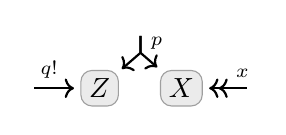
\begin{tikzpicture}[center base]
			\node[dpad0] (Z) {$Z$};
			\node[dpad0,right=.5 of Z] (X) {$X$};
			\coordinate (A) at ($ (X)!.5!(Z) + (0,0.7)$);
			\draw[arr1] (A) -- node[right]{$\scriptstyle p$} ++(0,-0.25) -- (X);
			\draw[arr1] (A) -- ++(0,-0.25) -- (Z);
%
			\draw[arr2, <<-] (X) --  node[above,pos=0.8]{$\scriptstyle x$} ++(0.9, 0);
			\draw[arr2, <-] (Z) -- node[above,pos=0.6]{$\scriptstyle q!$} ++(-0.9, 0);%
			%\scriptstyle q^{\{\beta =\infty\}}
			% \ar[r,"p"] \& Z \ar[r,"p", bend left] \& X \ar[l,"q", bend left] \& \ar[l, two heads, "x"']
		\end{tikzpicture}
		}%_{\!\!0}
% 		\right)
		.
	\]
\end{linked}



%
% The proof of \cref{prop:pdg-elbo-x} %, lke that of \cref{prop:pdg-Ix},
%  hinges critically on the fact that we force a single sample $x$; its PDG does not capture the whole context $\xsamp$.
% Nevertheless, we get an analogous result when we replace the sample $x$ with the entire data distribution $\datadist\xsamp$, which differs only in that the expression is offset by the entropy of the data distribution.
%
%
% \begin{prop}\label{prop:pdg-elbo-X}
% 	Consider a model $p(X,Z)$, auxiliary distribution $q(Z)$, and samples $\xsamp = \{x^{(i)}\}$ defining a data distribution $\datadist\xsamp$.
% 	The following are equal:
% 	\begin{enumerate}[label=(\arabic*)]
% 		\item $- \Ex_{\datadist\xsamp} \mathrm{ELBO}_{p,q}(X)$
% 		\item $\displaystyle\bbr{\,p\,}(q \otimes \datadist\xsamp) + \H(\datadist\xsamp)$
% 		\item \(\displaystyle%\lim_{\beta_q, \beta_{\datadist\xsamp} \to \infty}
% 			% \lim_{t \to \infty}
% 		  \aar[\Bigg]{
% 		  \begin{tikzpicture}[center base]
% 	  		\node[dpad0] (Z) {$Z$};
% 	  		\node[dpad0,right=.5 of Z] (X) {$X$};
% 	  		\coordinate (A) at ($ (X)!.5!(Z) + (0,0.7)$);
% 	  		\draw[arr1] (A) -- node[right]{$\scriptstyle p$} ++(0,-0.25) -- (X);
% 	  		\draw[arr1] (A) -- ++(0,-0.25) -- (Z);
% 	  %
% 	  		\draw[arr1, <-] (X) --  node[above,pos=0.2,anchor=south west]{$\scriptstyle {\datadist\xsamp}!$} ++(0.9, 0);
% 	  			% ^{\{\beta=\beta_0\}}
% 	  		\draw[arr1, <-] (Z) -- node[above]{$\scriptstyle q! $} ++(-0.9, 0);
% 	  	\end{tikzpicture} }_1 + \H(\datadist\xsamp)\)
% 	\end{enumerate}
%
% \end{prop}
% \begin{proof}
%
% \end{proof}



The use of the ELBO as an objective is often justified by the fact that it lower-bounds the objective that you ``really wanted'': the cross entropy.
This is often proved by jensen's inequality, or alternatively, but appeal to the non-negativity of relative entropy \cite{elboproofs}.
We now give a very simple, different-looking diagrammatic proof of this second approach, by appealing to the intuitive fact that adding believing more things cannot make you less inconsistent, as captured by \cref{lemma!}.

\[
\log \frac{1}{p(x)} =
    % \lim_{t \to \infty}
	 \aar[\Bigg]{
% 	  \Inc\left(
		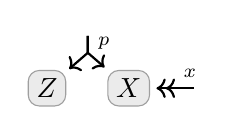
\begin{tikzpicture}[center base]
			\node[dpad0] (Z) {$Z$};
			\node[dpad0,right=.5 of Z] (X) {$X$};
			\coordinate (A) at ($ (X)!.5!(Z) + (0,0.7)$);
			\draw[arr1] (A) -- node[right]{$\scriptstyle p$} ++(0,-0.25) -- (X);
			\draw[arr1] (A) -- ++(0,-0.25) -- (Z);
%
			\draw[arr2, <<-] (X) --  node[above,pos=0.8]{$\scriptstyle x$} ++(0.9, 0);
% 			\draw[arr2, <-] (Z) -- node[above,pos=0.6]{$\scriptstyle q^{\{\beta =\infty\}}$} ++(-0.9, 0);%
			% \ar[r,"p"] \& Z \ar[r,"p", bend left] \& X \ar[l,"q", bend left] \& \ar[l, two heads, "x"']
		\end{tikzpicture}
		}%_{\!\!0}
% 		\right)
	\le
    % \lim_{t \to \infty}
	 \aar[\Bigg]{
% 	  \Inc\left(
		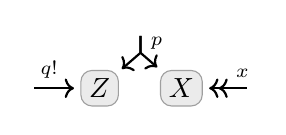
\begin{tikzpicture}[center base]
			\node[dpad0] (Z) {$Z$};
			\node[dpad0,right=.5 of Z] (X) {$X$};
			\coordinate (A) at ($ (X)!.5!(Z) + (0,0.7)$);
			\draw[arr1] (A) -- node[right]{$\scriptstyle p$} ++(0,-0.25) -- (X);
			\draw[arr1] (A) -- ++(0,-0.25) -- (Z);
%
			\draw[arr2, <<-] (X) --  node[above,pos=0.8]{$\scriptstyle x$} ++(0.9, 0);
			\draw[arr2, <-] (Z) -- node[above,pos=0.6]{$\scriptstyle q!$} ++(-0.9, 0);%
			% \ar[r,"p"] \& Z \ar[r,"p", bend left] \& X \ar[l,"q", bend left] \& \ar[l, two heads, "x"']
		\end{tikzpicture}
		}%_{\!\!0}
% 		\right)
    = -\mathrm{ELBO}_{p,q}(x),
\]

The first and last equalities are \Cref{prop:marginal-ll,prop:pdg-elbo-x} respectively, and
the inequality is an instance of \Cref{lemma!}.
We submit that this proof is more intuitve and gives a clearer picture of why it should be true. The second PDG has more edges, so it must be at least as inconsistent.
Furthermore, this picture shows us that if we simultaneously vary $q(Z)$ within an expressive enough class of distributions, the inequality is also tight, because the distribution that realizes the smallest inconsistency must have some marginal on $Z$ --- and taking $q$ to be that distribution will incur no additional inconsistency.


 We also have analog analog holds for the entire dataset at once, which is more easily formulated with a slightly different variational form in the next section.

% \begin{align*}
% \ell(p;\xsamp) &=
% 	 \aar[\Bigg]{
% 	 % \Inc\left(
% 		\begin{tikzpicture}[center base]
% 			\node[dpad0] (Z) {$Z$};
% 			\node[dpad0,right=.5 of Z] (X) {$X$};
% 			\coordinate (A) at ($ (X)!.5!(Z) + (0,0.7)$);
% 			\draw[arr1] (A) -- node[right]{$\scriptstyle p$} ++(0,-0.25) -- (X);
% 			\draw[arr1] (A) -- ++(0,-0.25) -- (Z);
% %
% 			\draw[arr1, <<-] (X) --  node[above,pos=0.8]{$\scriptstyle \datadist\xsamp$} ++(0.9, 0);
% 			% \draw[arr1, <-] (Z) -- node[above]{$\scriptstyle q$} ++(-0.9, 0);
% 		\end{tikzpicture}
% 		}%_{\!\!0}
% 		% \right)
% 		 + \H(\datadist\xsamp) \\
% 		&\le
% 			\lim_{t \to \infty}
% 		  \aar[\Bigg]{
% 		  \begin{tikzpicture}[center base]
% 	  		\node[dpad0] (Z) {$Z$};
% 	  		\node[dpad0,right=.5 of Z] (X) {$X$};
% 	  		\coordinate (A) at ($ (X)!.5!(Z) + (0,0.7)$);
% 	  		\draw[arr1] (A) -- node[right]{$\scriptstyle p$} ++(0,-0.25) -- (X);
% 	  		\draw[arr1] (A) -- ++(0,-0.25) -- (Z);
% 	  %
% 	  		\draw[arr1, <-] (X) --  node[above,pos=0.2,anchor=south west]{$ {\datadist\xsamp}^{\{\beta= t\}}$} ++(0.9, 0);
% 	  			% ^{\{\beta=\beta_0\}}
% 	  		\draw[arr1, <-] (Z) -- node[above]{$q^{\{\beta= t\}} $} ++(-0.9, 0);
% 	  	\end{tikzpicture} } + \H(\datadist\xsamp) = - \Ex_{\datadist\xsamp} \mathrm{ELBO}_{p,q}(X),
% \end{align*}
% which holds for the same reason.


\subsection{Variational Auto-Encoders and PDGs}

An autoencoder is a probabilistic model intended to compress a variable $X$ (e.g., an image) to a compact latent representation $Z$ (a compact vector), and is specified by two conditional distributions:
an encoder $e(Z \mid X)$, and a decoder $d(X \mid Z)$.
Of course, not all pairs of cpds fill this role equally well.
Perhaps most importantly, we would to have low \emph{reconstruction error} \eqref{eq:rec}---when we decode an encoded image, we would like it to be reasonably similar to the original.

\begin{equation}
 \mathrm{Rec}(x) = \Ex_{z \sim e \mid x} \underbrace{~\mathrm I_{d\mid z}(x)~}_{\substack{\text{Additional bits to}\\\text{specify $x$ from $d|z$}}}
	= \sum_z e(z \mid x) \log \frac1{d(x \mid z)}\label{eq:rec}
\end{equation}

% Note the similarity to the cross entropy objective from before, except in place of our

There are other desiderata as well. It would be nice if the distribution on $Z$ had a nice form---perhaps factoring into independent features, which we might use to describe $X$. We encode this wish in the form of a that $Z$ is distributed according to our favorite $p(Z)$, known as a variational prior.

In the autoencoding setting, $e$ functions as a variational approximation to the latent variable $Z$, differing from $q(Z)$ of the previous section only in that it can depend on $X$. Here, the analogue of the ELBO becomes
\begin{align*}
	\mathrm{ELBO}_{p,e,d}(x) &= \Ex_{z \sim e|x} \left[\log \frac{p(z) d(x\mid z)}{e(z\mid x)} \right] \\
		&= \Ex_{z \sim e|x}\left[ \log \frac{p(z)}{e(z\mid x)}  \right] - \Ex_{z \sim e|x} \left[\log \frac1{d(x\mid z)} \right] \\
		&= \kldiv{e(Z|x)}{p} - \mathrm{Rec}(x).
\end{align*}

This gives us the following results, analogous to \cref{prop:pdg-elbo-x}.

\begin{linked}{prop}{pdg-elbo-vae}
	The conditional ELBO used as a VaE objective is the inconsistency of the PDG containing the encoder $e$, decoder $d$ prior $p$, and a sample $x$.
	That is,
	\[
	-\mathrm{ELBO}_{p,e,d}(x) =
	 \aar*{
		% \begin{tikzcd}[AmpRep,row sep=1em,column sep=1.5em]
		% 	\ar[r,"p"] \& Z \ar[r,"d", bend left] \& X \ar[l,"e!", bend left] \& \ar[l, two heads, "x"']
		% \end{tikzcd}
		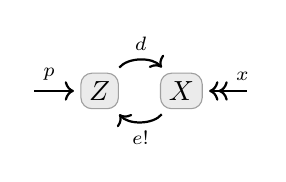
\begin{tikzpicture}[center base]
			\node[dpad0] (Z) {$Z$};
			\node[dpad0,right=.5 of Z] (X) {$X$};
			\draw[arr2, ->] (X) to[bend left=50]
				node[below]{$\scriptstyle e!$} (Z);
			\draw[arr2, ->] (Z) to[bend left=50]
				node[above]{$\scriptstyle d$} (X);
			\draw[arr2, <<-] (X) --
			  	node[above,pos=0.8]{$\scriptstyle x$}
			 	++(0.9, 0);
			\draw[arr2, <-] (Z) --
				node[above,pos=0.6]{$\scriptstyle p$}
				++(-0.9, 0);%
		\end{tikzpicture}}
	\]
\end{linked}
\begin{linked}{prop}{pdg-elbo-vae-whole}
	The following analog of \cref{prop:pdg-elbo-vae} for a whole dataset $\xsamp$ holds:
	\[
	-\Ex_{\datadist\xsamp}\mathrm{ELBO}_{p,e,d}(X) =
	 \aar*{
		% \begin{tikzcd}[AmpRep,row sep=1em,column sep=1.5em]
		% 	\ar[r,"p"] \& Z \ar[r,"d", bend left] \& X \ar[l,"e!", bend left] \& \ar[l, two heads, "x"']
		% \end{tikzcd}
		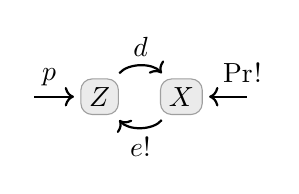
\begin{tikzpicture}[center base]
			\node[dpad0] (Z) {$Z$};
			\node[dpad0,right=.5 of Z] (X) {$X$};
			\draw[arr2, ->] (X) to[bend left=50]
				node[below]{$e!$} (Z);
			\draw[arr2, ->] (Z) to[bend left=50]
				node[above]{$d$} (X);
			\draw[arr2, <-] (X) --
				node[above,pos=0.8]{$\datadist\xsamp!$}
				++(0.9, 0);
			\draw[arr2, <-] (Z) --
				node[above,pos=0.6]{$p$}
				++(-0.9, 0);%
		\end{tikzpicture}} + \H(\datadist\xsamp). \]
\end{linked}


\subsubsection{Intuitive Proofs of Variational Bounds}
\Cref{prop:pdg-elbo-vae,prop:pdg-elbo-vae-whole} can be used to derive the variational lower bound. Once again, the addition of the edge $e$ cannot decrease the inconsistency (\cref{lemma!}), but it makes it easier to identify and sample from the best-scoring distributions.
This result in the following simple visual proof:
\[
	- \log \Pr(x) =
	\aar*{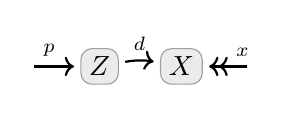
\begin{tikzpicture}[center base]
	   \node[dpad0] (Z) {$Z$};
	   \node[dpad0,right=.5 of Z] (X) {$X$};
	   \draw[arr2, ->] (Z) to[bend left=10]
		   node[above]{$\scriptstyle d$} (X);
	   \draw[arr2, <<-] (X) --
		   node[above,pos=0.8]{$\scriptstyle x$}
		   ++(0.9, 0);
	   \draw[arr2, <-] (Z) --
		   node[above,pos=0.6]{$\scriptstyle p$}
		   ++(-0.9, 0);%
	\end{tikzpicture}}
 	\le
 	\aar*{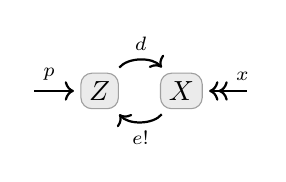
\begin{tikzpicture}[center base]
		\node[dpad0] (Z) {$Z$};
		\node[dpad0,right=.5 of Z] (X) {$X$};
		\draw[arr2, ->] (X) to[bend left=50]
			node[below]{$\scriptstyle e!$} (Z);
		\draw[arr2, ->] (Z) to[bend left=50]
			node[above]{$\scriptstyle d$} (X);
		\draw[arr2, <<-] (X) --
			node[above,pos=0.8]{$\scriptstyle x$}
			++(0.9, 0);
		\draw[arr2, <-] (Z) --
			node[above,pos=0.6]{$\scriptstyle p$}
			++(-0.9, 0);%
	\end{tikzpicture}} = -\mathrm{ELBO}_{p,e,d}(x).
\]
Here $\Pr(X)$ is the marginal of $p(Z)d(X \mid Z)$ on $X$.
\Cref{prop:many-equal-simple,prop:pdg-elbo-vae-whole} lets us do the same thing for many i.i.d. datapoints at once, with only a single application of the inequality:
\begin{align*}
	- \log \Pr(\xsamp) = - \log \prod_{i=1}^m \left(\Pr(x^{(i)})\right) =
	- \frac1{m}\sum_{i = 1}^m \log \Pr(x^{(i)})   = &\\
	\H(\datadist\xsamp) + \aar*{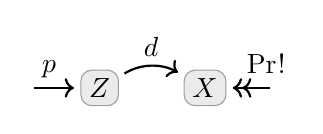
\begin{tikzpicture}[center base]
	   \node[dpad0] (Z) {$Z$};
	   \node[dpad0,right=0.8 of Z] (X) {$X$};
	   \draw[arr2, ->] (Z) to[bend left=30]
		   node[above]{$d$} (X);
	   \draw[arr2, <<-] (X) --
		   node[above,pos=0.8]{$\datadist\xsamp!$}
		   ++(0.9, 0);
	   \draw[arr2, <-] (Z) --
		   node[above,pos=0.6]{$p$}
		   ++(-0.9, 0);%
	\end{tikzpicture}}
 	&\le
 	\aar*{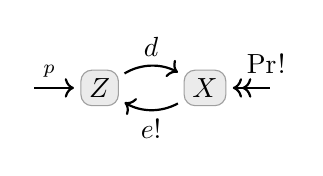
\begin{tikzpicture}[center base]
		\node[dpad0] (Z) {$Z$};
		\node[dpad0,right=.8 of Z] (X) {$X$};
		\draw[arr2, ->] (X) to[bend left=30]
			node[below]{$e!$} (Z);
		\draw[arr2, ->] (Z) to[bend left=30]
			node[above]{$d$} (X);
		\draw[arr2, <<-] (X) --
			node[above,pos=0.8]{$\datadist\xsamp!$}
			++(0.9, 0);
		\draw[arr2, <-] (Z) --
			node[above,pos=0.6]{$\scriptstyle p$}
			++(-0.9, 0);%
	\end{tikzpicture}} + \H(\datadist\xsamp) \\
	&\qquad\qquad= -\Ex_{\datadist\xsamp}\mathop{\mathrm{ELBO}}\limits_{p,e,d}(X)
\end{align*}
\subsection{\texorpdfstring{$\beta$}{beta}-VaE Objective}

The ELBO is not the only objective that has been considered to train VaEs.
In the most common variant, Higgins et. al. \cite{higgins2016beta} have argued that the one might want to weight the reconstruction loss (from \eqref{eq:rec}) and KL term differently.  They suggest an objective of the form
\[ \beta\text{-}\mathrm{ELBO}_{p,e,d}(x) := \mathrm{Rec}(x) - \beta \kldiv{e(Z|x)}{p}\]
which for $\beta = 1$ is equivalent to the ELBO from the previous section. The authors view it as a regularization parameter, annd argue that in some cases, you can do better with a stronger prior. Sure enough, this extra parameter corresponds to the confidence of $p$, which also happens go by the same name.\footnote{the two terms actually both share an origin in thermodynamic $\beta$ for inverse temperature.}

\begin{linked}{prop}{beta-elbo}
	The negative $\beta$-ELBO objective for a prior $p(X)$, encoder $e(Z \mid X)$, decoder $d(X \mid Z)$, at a sample $x$, is equal to the inconsistency of the corresponding PDG, where the prior has confidence equal to $\beta$. That is,
	\[
	-\beta\text{-}\mathrm{ELBO}_{p,e,d}(x) =
	 \aar**{
		% \begin{tikzcd}[AmpRep,row sep=1em,column sep=1.5em]
		% 	\ar[r,"p"] \& Z \ar[r,"d", bend left] \& X \ar[l,"e!", bend left] \& \ar[l, two heads, "x"']
		% \end{tikzcd}
		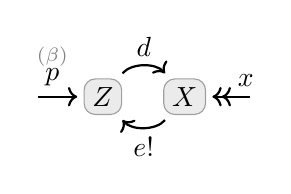
\begin{tikzpicture}[center base]
			\node[dpad0] (Z) {$Z$};
			\node[dpad0,right=.5 of Z] (X) {$X$};
			\draw[arr2, ->] (X) to[bend left=50]
				node[below]{$ e!$} (Z);
			\draw[arr2, ->] (Z) to[bend left=50]
				node[above]{$ d$} (X);
			\draw[arr2, <<-] (X) --
			  	node[above,pos=0.8]{$ x$}
			 	++(0.9, 0);
			\draw[arr2, <-] (Z) --
				node[above,pos=0.6]{$ \overset{{\color{gray}(\beta)}}p$}
				++(-0.9, 0);%
		\end{tikzpicture}}
	\]
\end{linked}



\section{Log Partition Function as Inconsistency}
The factors of a factor graph, which in isolation indicate relative probabilities.
Factored exponential families form the mathematical backbone of statistical
mechanics, in which the normalization constant
$Z_{\Psi}$ for the WFG $\Psi = (\phi_j, \theta_j)_{j \in \cal J}$,
given by
$$
	Z_{\Psi} := \sum_{\mat w} \prod_{j \in \mathcal J} \phi_j(\mat w_j)^{\theta_j}
	,
$$
is known as the \emph{partition function}. If every factor is a cpd, and every variable has at least one incoming edge, then $Z_\Psi$ is at most 1, so $-\log Z_\Psi$ is non-negative, and measures how far away the product of factors is from being normalized. Thus, it is in some sense a measure of inconsistency of a factor graph.
It turns out that this intuition coincides with our notion of PDG inconsistency.

\begin{linked}{prop}{fg-inconsistency-is-partition-function}
	For any weighted factor graph
	$\Psi$, we have $\aar{\PDGof{\Psi}}_1 = - \log Z_{\Psi}$.
\end{linked}

Many thermodynamic quantities
(e.g., as internal energy, free energy, pressure, volume, and entropy) can
be obtained by taking various partial derivatives of $Z_\Psi$, and calculating the partition function is closely related to infering marginal distributions \cite{}.

\section{Discussion}

\textbf{Inconsistency, in a different light.}
Nobody likes building broken things, and so those of who build systems commonly try to eliminate it in models by design. But in doing so, we unwittingly sacrifice tools for dealing with it if (and when) it does arise.


\textbf{A Universal Objective.}
Objective functions in machine learning are often quite opaque to new-comers.
Only a few of them are especially common, and they are often presented in an ad hoc way; there are many loss functions that have the properties we need to train networks. So why do we lean so heavily on a few select choices (dependent on the problem setup), such as the cross entropy, and the ELBO objective?
PDGs provide one answer to this question.

There is perhaps a more important argument for using PDGs over other models. By designing a model, rather than an objective function, it is easier to understand what the pieces are, what is and is not relevant to the task, and no longer possible to twiddle with the objective until you get the results you want --- you can only twiddle with the model, where hacks are more easily spotted.

\textbf{Semantics for ``Graphical Models''.}
Often, autoencoder tutorials will include diagrams, and falsely claim that they are standard ``graphical models''. In these cases, among others, people are already reasoning about local probabilistic information in a graph. We have shown here that PDG semantics can sense of these informal diagrams in a way that is deeply connected with the variational reasoning involed.

\bibliographystyle{plain}
\bibliography{refs}

\clearpage
\appendix
\section{Proofs}


\recall{prop:pdg-Ix}
% \csname prop:pdg-Ix\endcsname*
\begin{lproof}\label{proof:pdg-Ix}
	Any distribution $\mu(X)$ that places mass on some $x' \ne x$ will have infinite KL divergence from the point mass on $x$. Thus, the only possibility for a finite consistency arises when $\mu = \delta_x$, and so
	\begin{equation*}
		\aar[\Big] {
		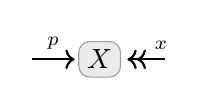
\begin{tikzpicture}[center base]
			\node[dpad0] (X) {$X$};
			\coordinate (A) at ($(X) + (-0.9,0)$);
			\draw[arr1] (A) -- node[above]{$\scriptstyle p$}  (X);
	%
			\draw[arr2, <<-] (X) --  node[above,pos=0.8]{$\scriptstyle x$} ++(0.9, 0);
		\end{tikzpicture}
		}
		= \bbr*{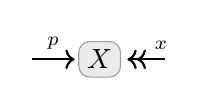
\begin{tikzpicture}[center base]
			\node[dpad0] (X) {$X$};
			\coordinate (A) at ($(X) + (-0.9,0)$);
			\draw[arr1] (A) -- node[above]{$\scriptstyle p$}  (X);
	%
			\draw[arr2, <<-] (X) --  node[above,pos=0.8]{$\scriptstyle x$} ++(0.9, 0);
		\end{tikzpicture}}( \delta_x )
		= \kldiv{\delta_x}{p} = \log \frac{1}{p(x)} = \I_p(x).
	\end{equation*}
\end{lproof}


\recall{prop:many-equal-simple}
\begin{lproof} \label{proof:many-equal-simple}
	The equality of 1 and 2 is standard. The equality of 3 and 4 can be seen by the fact that in the limit of infinite confidence on $\datadist\xsamp$, the optimal distribution must also equal $\datadist\xsamp$, so the least inconsistency is attained at this value.
	Finally it remains to show that the first two and last two are equal:
	\begin{align*}
		\bbr{\,p\,}_\gamma(\datadist\xsamp) + (1+\gamma)\H(\datadist\xsamp)
		&=  \kldiv{\datadist\xsamp}{p} - \gamma \H(\datadist\xsamp)+ (1+\gamma)\H(\datadist\xsamp) \\
		&= \kldiv{\datadist\xsamp}{p} + \H(\datadist\xsamp) \\
		&= \Ex\nolimits_{\datadist\xsamp}\left[\log\frac{\datadist\xsamp}{p} +  \log\frac{1}{\datadist\xsamp}\right]
		= \Ex\nolimits_{\datadist\xsamp}\left[\log\frac{1}{p}\right],
	\end{align*}
	which is the cross entropy, as desired.
\end{lproof}


\recall{prop:marginal-ll}
\begin{lproof}\label{proof:marginal-ll}
	As before, all mass of $\mu$ must be on $x$ for it to have a finite score.
	Thus it suffices to consider joint distributions of the form $\mu(X,Z) = \delta_x(X) \mu(Z)$.
	We have
	\begin{align*}
	\aar*{
		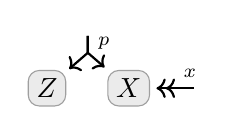
\begin{tikzpicture}[center base]
			\node[dpad0] (Z) {$Z$};
			\node[dpad0,right=.5 of Z] (X) {$X$};
			\coordinate (A) at ($ (X)!.5!(Z) + (0,0.7)$);
			\draw[arr1] (A) -- node[right]{$\scriptstyle p$} ++(0,-0.25) -- (X);
			\draw[arr1] (A) -- ++(0,-0.25) -- (Z);
			\draw[arr2, <<-] (X) --  node[above,pos=0.8]{$\scriptstyle x$} ++(0.9, 0);
		\end{tikzpicture}}
			&= \inf_{\mu(Z)} \bbr*{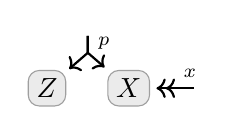
\begin{tikzpicture}[center base]
				\node[dpad0] (Z) {$Z$};
				\node[dpad0,right=.5 of Z] (X) {$X$};
				\coordinate (A) at ($ (X)!.5!(Z) + (0,0.7)$);
				\draw[arr1] (A) -- node[right]{$\scriptstyle p$} ++(0,-0.25) -- (X);
				\draw[arr1] (A) -- ++(0,-0.25) -- (Z);
				\draw[arr2, <<-] (X) --  node[above,pos=0.8]{$\scriptstyle x$} ++(0.9, 0);
			\end{tikzpicture}}\Big(\delta_x(X)\mu(Z)\Big)  \\
			&= \inf_{\mu(Z)}\kldiv[\Big]{\delta_x(X)\mu(Z)}{p(X,Z)} \\
			&= \inf_{\mu(Z)}\Ex_{z \sim \mu} \log \frac{\mu(z)}{p(x,z)}
			~= \inf_{\mu(Z)}\Ex_{z \sim \mu} \log \frac{\mu(z)}{p(x,z)}\frac{p(x)}{p(x)} \\
			&= \inf_{\mu(Z)}\Ex_{z \sim \mu} \left[ \log \frac{\mu(z)}{p(z \mid x)} + \log \frac{1}{p(x)} \right] \\
			&= \inf_{\mu(Z)} \Big[\kldiv{\mu(Z)}{p(Z\mid x)}\Big] + \log \frac{1}{p(x)} \\
			&= \log \frac{1}{p(x)} = \I_p(x) & \text{[Gibbs Inequality]}
	\end{align*}
\end{lproof}

\recall{prop:pdg-loglikelihood}
\begin{lproof}\label{proof:pdg-loglikelihood}
	The same idea as in \cref{prop:marginal-ll}, but a little more complicated.

	\begin{align*}
	\aar*{
		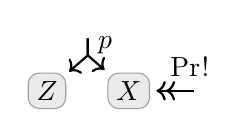
\begin{tikzpicture}[center base]
			\node[dpad0] (Z) {$Z$};
			\node[dpad0,right=.5 of Z] (X) {$X$};
			\coordinate (A) at ($ (X)!.5!(Z) + (0,0.7)$);
			\draw[arr1] (A) -- node[right]{$p$} ++(0,-0.25) -- (X);
			\draw[arr1] (A) -- ++(0,-0.25) -- (Z);
			\draw[arr2, <<-] (X) --  node[above,pos=0.8]{$\datadist\xsamp!$} ++(0.9, 0);
		\end{tikzpicture}}
			&= \inf_{\mu(Z \mid X)} \bbr*{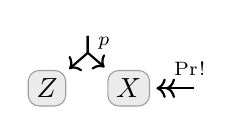
\begin{tikzpicture}[center base]
				\node[dpad0] (Z) {$Z$};
				\node[dpad0,right=.5 of Z] (X) {$X$};
				\coordinate (A) at ($ (X)!.5!(Z) + (0,0.7)$);
				\draw[arr1] (A) -- node[right]{$\scriptstyle p$} ++(0,-0.25) -- (X);
				\draw[arr1] (A) -- ++(0,-0.25) -- (Z);
				\draw[arr2, <<-] (X) --  node[above,pos=0.8]{$\scriptstyle \datadist\xsamp!$} ++(0.9, 0);
			\end{tikzpicture}}\Big(\datadist\xsamp(X) \mu(Z \mid X)\Big)  \\
			&= \inf_{\mu(Z \mid X)}\kldiv[\Big]{\datadist\xsamp(X) \mu(Z \mid X)}{p(X,Z)} \\
			&= \inf_{\mu(Z \mid X)}
				\Ex_{\substack{x \sim \datadist\xsamp \\ z \sim \mu}}
					\log \frac{\mu(z \mid x)\datadist\xsamp(x)}{p(x,z)} \\
			&= \frac{1}{|\xsamp|}\inf_{\mu(Z\mid X)}\sum_{x \in \xsamp}
				\Ex_{z \sim \mu(Z\mid x)} \log \frac{\mu(z \mid x) \datadist\xsamp(x) }{p(x,z)}\frac{p(x)}{p(x)} \\
			&= \frac{1}{|\xsamp|}\inf_{\mu(Z \mid X)}\sum_{x \in \xsamp}\Ex_{z \sim \mu} \left[ \log \frac{\mu(z)}{p(z \mid x)} + \log \frac{1}{p(x)} - \log \frac{1}{\datadist\xsamp(x)} \right] \\
			&= \frac{1}{|\xsamp|}\sum_{x \in \xsamp} \left[
				\inf_{\mu(Z)} \Big[\kldiv{\mu(Z)}{p(Z\mid x)}\Big] + \log \frac{1}{p(x)} \right] - \H(\datadist\xsamp) \\
			&= \frac{1}{|\xsamp|}\sum_{x \in \xsamp} \log \frac{1}{p(x)} - \H(\datadist\xsamp)
			= \frac{1}{|\xsamp|} \sum_{x \in \xsamp} I_p(x) - \H(\datadist\xsamp) \\
			\Big(\quad&= \kldiv{\datadist\xsamp}{p(X)} \quad \Big)
	\end{align*}
\end{lproof}


\recall{prop:supervised-cross-entropy}
\begin{lproof} \label{proof:supervised-cross-entropy}
	$\datadist\xysamp$ has high confidence, it is the only joint distribution $\mu$ with finite score. Since $f$ is the only other edge, the inconsistency is therefore
	\begin{align*}
	\Ex_{x \sim \datadist\xysamp} \kldiv[\Big]{\datadist\xysamp(Y\mid x)}{f(Y\mid x)}
		&= \Ex_{x,y \sim \datadist\xysamp} \left[\log \frac{\datadist\xysamp(y\mid x)}{f(y\mid x)}\right]\\
		&= \Ex_{x,y \sim \datadist\xysamp} \left[ \log \frac{1}{f(y\mid x)} - \log \frac{1}{\datadist\xysamp(y\mid x)} \right] \\
		&= \frac1{|\xysamp|}\sum_{(x,y) \in \xysamp} \left[\log \frac1{f(y \mid x)}\right] \quad - \H_{\datadist\xysamp}(Y\mid X)
	\end{align*}
	\[  \]
\end{lproof}

\recall{prop:accuracy}
\begin{lproof}\label{proof:accuracy}
	Becuase $f$ is deterministic, for every $x$ in the support of a joint distribution $\mu$ with finite score, we must have $\mu(Y\mid x) = \delta_f$, since if $\mu$ were to place any non-zero mass $\mu(x,y) = \epsilon > 0$  on a pont $(x,y)$ with $y \ne f(x)$ results in an infinite contribution to the KL divergence
	\[ \kldiv{\mu(Y\mid x)}{\delta_{f(x)}} =
	 	\Ex_{x,y \sim \mu} \log \frac{\mu(y\mid x)}{\delta_{f(x)}} \ge \mu(y,x) \log \frac{\mu(x,y)}{\mu(x) \cdot \delta_{f(x)}(y)} =  \epsilon \log \frac{\epsilon}{0} = \infty.
	\]
	The same holds for $h$. Therefore, for any $\mu$ with a finite score, and $x$ with $\mu(x) > 0$, we have $\delta_{f(x)} = \mu(Y\mid x) =  \delta_{h(x)}$, meaning that we need only consider $\mu$ whose support is a subset of those points on which $f$ and $h$ agree.
	On all such points, the contribution to the score from the edges associated to $f$ and $h$ will be zero, since $\mu$ matches the conditional marginals exactly, and the total incompatibility of such a distribution $\mu$ is equal to the relative entropy $\kldiv{\mu}{D}$, scaled by the confidence $\beta$ of the emperical distribution $D$.

	So, among those distributions $\mu(X)$ supported on an event $E \subset \V (X)$, which minimizes is the relative entropy of $\kldiv{\mu}{D}$?
	It is well known that the conditional distribution
	% $D \mid E \propto \mathbbm1[E] D(X) = \frac{1}{D(E)} \mathbbm1[E] D(X) $
	$D \mid E \propto \delta_E(X) D(X) = \frac{1}{D(E)} \delta_E(X) D(X) $
	 satisfies this property uniquely (see, for instance, \cite{halpernRAU}). Let $f\!=\!h$ denote the event that $f$ and $h$ agree. Then we calculate
	\begin{align*}
		\aar*{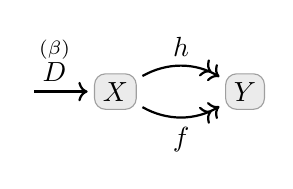
\begin{tikzpicture}[center base]
				\node[dpad0] (Y) {$Y$};
				\node[dpad0,left=1.1 of Y] (X) {$X$};
				%
				\draw[arr2, ->>] (X) to[bend left] node[pos=0.5, above]{$h$} (Y);
				\draw[arr2, ->>] (X) to[bend right] node[pos=0.5, below]{$f$} (Y);
				\draw[arr2, <-] (X) to node[pos=0.6, above]{$\overset{(\beta)}D$} +(-1.1, 0);
			\end{tikzpicture}}
		&=  \!\! \inf_{\substack{\mu(X)~\text{s.t.} \\ { \mathrm{supp}(\mu) \subseteq [f=h]}} } \beta \kldiv[\Big]{\mu(X)}{D(X)} \\
		&= \beta \kldiv[\Big]{ D \mid [f\!=\!h]}{ D } \\
		&= \beta \Ex_{D \mid f=h}
			\log \frac
				% {\mathbbm1[f\!=\!h](X)  D(X)}
				{\delta_{f=h}(X)  D(X)}
				{D(f\!=\!h)\cdot D(X)} \\
		&= \beta \Ex_{ D \mid f=h} \log \frac{1}{D(f\!=\!h)}
			& \hspace{-2em}{\color{gray}\left[ \begin{tabular}{c}
				% since $\mathbbm1[f\!=\!h](x) = 1$ for all $x$  that \\
				since $\delta_{f=h}(x) = 1$ for all $x$  that \\
				 contribute to the expectation \end{tabular} \right]} \\
		%&=	\inf_{\mu(X)} \Ex_{x \sim \mu} \beta \log \frac{\mu(x)}{D(x)} \\
		&= - \beta\, \log D(f=h)
			&  {\color{gray}\left[ \begin{tabular}{c}since $D(f=h)$ is a constant \end{tabular} \right]} \\
		&= - \beta\,\log \Big( \mathrm{accuracy}_{f,D} (h) \Big)\\
		&=  \beta\, \I_D[f=h].
	\end{align*}
\end{lproof}

\recall{prop:inc-two-gaussians}
\begin{lproof}\label{proof:inc-two-gaussians}
	Let $\dg M$ denote the PDG in question.
	%To simplify notation and emphasize their roles, we will write $\mu_1$ in place of $f(x)$, $\sigma_1$ in place of $t(x)$, and so forth.
	Since $D$ has high confidence, we know any joint distribution $\mu$ with a finite score must have $\mu(X) = D(X)$. Thus,
	\begin{align*}
		\aar{\dg M}_0 &= \inf_\mu \Ex_{x\sim D}\Ex_{y \sim\mu|x}
		 	\left[ \beta_1 \log \cfrac
				{\mu(y \mid x)}
				{\mathcal N(y \mid f(x), t(x))}
				%
				+  \beta_2 \log \cfrac
					{\mu(y \mid x)}
					{\mathcal N(y \mid h(x), s(x))}
				\right] \\
			&= \inf_\mu \Ex_{x\sim D}\Ex_{y \sim\mu|x}
			 	\left[ \beta_1 \log \frac
					{\mu(y \mid x)}
					{\frac{1}{t(x) \sqrt{2\pi}} \exp\left( -\frac{1}{2} \left(\frac{y-f(x)}{t(x)}\right)^2\right)}
					%
					+  \beta_2 \log \frac
						{\mu(y \mid x)}
						{\frac{1}{s(x) \sqrt{2\pi}} \exp\left( -\frac{1}{2} \left(\frac{y-h(x)}{s(x)}\right)^2\right)}
					\right] \\
			&= \inf_\mu \Ex_{x\sim D}\Ex_{y \sim\mu|x}
			 	\left[ \log \mu(y \mid x)^{\beta_1 + \beta_2}
					\begin{array}{l}
					+ \beta_1 \log( t(x) \sqrt{2\pi}) + \frac{\beta_1}{2} \left( \frac{y-f(x)}{t(x)} \right)^2\\
					+ \beta_2 \log( t(x) \sqrt{2\pi}) + \frac{\beta_2}{2} \left( \frac{y-h(x)}{s(x)} \right)^2
					\end{array}
					\right] \\
	\end{align*}

	\todo
\end{lproof}

\recall{lemma:pdgdiv}
\begin{lproof}\label{proof:pdgdiv}
	\begin{align*}
	\aar[\bigg]{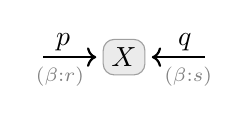
\begin{tikzpicture}[center base]
		\node[dpad0] (X) {$X$};
		\draw[arr2, <-] (X) --
				% node[above] {$\overset{(\beta : r)}p$}
				node[above, pos=0.6, inner sep=2pt, align=center] {$p$}
				node[below, pos=0.65, inner sep=3pt, align=center] {$\scriptstyle{\color{gray}(\beta : r)}$}
			++(-1.1,0);
		\draw[arr2, <-] (X) --
				% node[above,pos=0.5] {$\overset{(\beta : s)}q$}
				node[above, pos=0.6, inner sep=2pt, align=center] {$q$}
				node[below, pos=0.65, inner sep=3pt, align=center] {$\scriptstyle{\color{gray}(\beta : s)}$}
			 ++(1.1, 0);
	\end{tikzpicture}}
	&= \inf_\mu \Ex_\mu \log \frac{\mu(x)^{r+s}}{p(x)^r q(x)^s}\\
	&= (r+s) \inf_\mu \Ex_\mu  \left[ \log \frac{\mu(x)}{(p(x)^r q(x)^s)^{\frac1{r+s}}} \cdot \frac{Z}{Z} \right] \\
	&= \inf_\mu (r+s) \kldiv*{\mu}{\frac1Z p^{\frac r{r+s}} q^{\frac s{r+s}}} - (r+s) \log Z\\
	\intertext{where $Z := (\sum_x p(x)^r q(x)^s)^{\frac1{r+s}}$ is the constant required to normalize the denominator as a distribution. Since this is now a relative entropy, it achives its minimum when $\mu$ is the other distribution, at which point it contributes zero, so our formula becomes}
	&= - (r+s) \log Z \\
	&= - (r+s) \log  \sum_x \left(p(x)^{r}\vphantom{\Big|} q(x)^{s}\right)^{\frac{1}{r+s}}
	\quad\text{as promised.}
	\end{align*}
\end{lproof}


\recall{prop:regularized}
\begin{lproof}\label{proof:regularized}
\end{lproof}

\recall{prop:pdg-elbo-x}
\begin{lproof}\label{proof:pdg-elbo-x}
	Every distribution that does marginalize to $q(Z)$ or places any mass on $x' \ne x$ will have infinite score. Thus the only distribution that could have a finite score is $\mu(X,Z)$. Thus,

	\begin{align*}
	\aar[\Bigg]{
% 	  \Inc\left(
	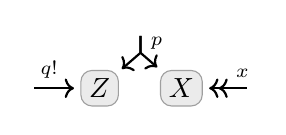
\begin{tikzpicture}[center base]
		\node[dpad0] (Z) {$Z$};
		\node[dpad0,right=.5 of Z] (X) {$X$};
		\coordinate (A) at ($ (X)!.5!(Z) + (0,0.7)$);
		\draw[arr1] (A) -- node[right]{$\scriptstyle p$} ++(0,-0.25) -- (X);
		\draw[arr1] (A) -- ++(0,-0.25) -- (Z);
%
		\draw[arr2, <<-] (X) --  node[above,pos=0.8]{$\scriptstyle x$} ++(0.9, 0);
		\draw[arr2, <-] (Z) -- node[above,pos=0.6]{$\scriptstyle q!$} ++(-0.9, 0);%
		%\scriptstyle q^{\{\beta =\infty\}}
		% \ar[r,"p"] \& Z \ar[r,"p", bend left] \& X \ar[l,"q", bend left] \& \ar[l, two heads, "x"']
	\end{tikzpicture}
	}
	 &= \inf_\mu \bbr*{
% 	  \Inc\left(
		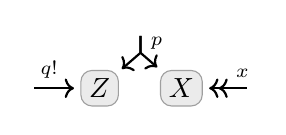
\begin{tikzpicture}[center base]
			\node[dpad0] (Z) {$Z$};
			\node[dpad0,right=.5 of Z] (X) {$X$};
			\coordinate (A) at ($ (X)!.5!(Z) + (0,0.7)$);
			\draw[arr1] (A) -- node[right]{$\scriptstyle p$} ++(0,-0.25) -- (X);
			\draw[arr1] (A) -- ++(0,-0.25) -- (Z);
%
			\draw[arr2, <<-] (X) --  node[above,pos=0.8]{$\scriptstyle x$} ++(0.9, 0);
			\draw[arr2, <-] (Z) -- node[above,pos=0.6]{$\scriptstyle q!$} ++(-0.9, 0);%
			%\scriptstyle q^{\{\beta =\infty\}}
			% \ar[r,"p"] \& Z \ar[r,"p", bend left] \& X \ar[l,"q", bend left] \& \ar[l, two heads, "x"']
		\end{tikzpicture}
		}( \mu ) \\
	  &= \bbr*{
 % 	  \Inc\left(
 		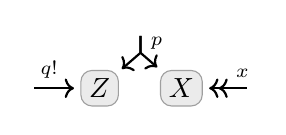
\begin{tikzpicture}[center base]
 			\node[dpad0] (Z) {$Z$};
 			\node[dpad0,right=.5 of Z] (X) {$X$};
 			\coordinate (A) at ($ (X)!.5!(Z) + (0,0.7)$);
 			\draw[arr1] (A) -- node[right]{$\scriptstyle p$} ++(0,-0.25) -- (X);
 			\draw[arr1] (A) -- ++(0,-0.25) -- (Z);
 %
 			\draw[arr2, <<-] (X) --  node[above,pos=0.8]{$\scriptstyle x$} ++(0.9, 0);
 			\draw[arr2, <-] (Z) -- node[above,pos=0.6]{$\scriptstyle q!$} ++(-0.9, 0);%
 			%\scriptstyle q^{\{\beta =\infty\}}
 			% \ar[r,"p"] \& Z \ar[r,"p", bend left] \& X \ar[l,"q", bend left] \& \ar[l, two heads, "x"']
 		\end{tikzpicture}
 		}( \delta_x(X) q(Z) ) \\
	 &= \Ex_{\substack{x' \sim \delta_x \\ z \sim q}} \log \frac{\delta_x(x')q(z)} {p(x',z)}
	 = - \Ex_{z \sim q} \frac{p(x,z)}{q(z)} = - \mathrm{ELBO}_{p,q}(x).
	\end{align*}
\end{lproof}

We proove both \Cref{prop:pdg-elbo-vae} and \cref{prop:pdg-elbo-vae-whole} at the same time.
\recall{prop:pdg-elbo-vae}
\recall{prop:pdg-elbo-vae-whole}
\begin{lproof}\label{proof:pdg-elbo-vae}\label{proof:pdg-elbo-vae-whole}
	The two proofs are similar. For \cref{prop:pdg-elbo-vae}, the optimal distribution must be $\delta_x(X) e(Z \mid X)$, and for \cref{prop:pdg-elbo-vae-whole}, it must be $\datadist\xsamp(X) e(Z \mid X)$, because $e$ and the data both have infinite confidence, so any other distribution gets an infinite score.
	At the same time, $d$ and $p$ define a joint distribution, so the inconsistency in question becomes
	\[
		\kldiv[\Big]{\delta_x(X) e(Z \mid X)}{p(Z)d(X\mid Z)}
			 = \Ex_{z \sim e \mid x} \left[ \log \frac{p(z)d(x\mid z)}{e(z \mid x)} \right] = \mathrm{ELBO}_{p,e,d}(x)
	\]
	in the first, case, and
	\begin{align*}
		\kldiv[\Big]{\datadist\xsamp(X) e(Z \mid X)}{p(Z)d(X\mid Z)}
		 &= \frac{1}{|\xsamp|}\sum_{x \in \xsamp} \Ex_{z \sim e \mid x} \left[ \log \frac{p(z)d(x\mid z)}{e(z \mid x)} + \log \frac{1}{\datadist\xsamp(x)} \right]\\
		 &= \mathrm{ELBO}_{p,e,d}(x) - \H(\datadist\xsamp)
	\end{align*}
	in the second.
\end{lproof}

\recall{prop:beta-elbo}
\begin{lproof} \label{proof:beta-elbo}
	\begin{align*}
		\aar*{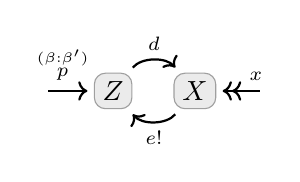
\begin{tikzpicture}[center base]
			\node[dpad0] (Z) {$Z$};
			\node[dpad0,right=.5 of Z] (X) {$X$};
			\draw[arr2, ->] (X) to[bend left=50]
			   node[below]{$\scriptstyle e!$} (Z);
			\draw[arr2, ->] (Z) to[bend left=50]
			   node[above]{$\scriptstyle d$} (X);
			\draw[arr2, <<-] (X) --
			   node[above,pos=0.8]{$\scriptstyle x$}
			   ++(0.9, 0);
			\draw[arr2, <-] (Z) --
			   node[above,pos=0.6]{$\scriptstyle \overset{(\beta : \beta')}p$}
			   ++(-0.9, 0);%
	   \end{tikzpicture}}
	   	&= \inf_\mu \bbr[\Bigg]{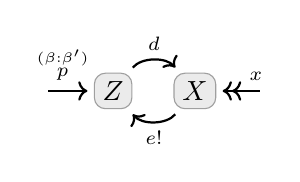
\begin{tikzpicture}[center base]
 		   \node[dpad0] (Z) {$Z$};
 		   \node[dpad0,right=.5 of Z] (X) {$X$};
 		   \draw[arr2, ->] (X) to[bend left=50]
 			   node[below]{$\scriptstyle e!$} (Z);
 		   \draw[arr2, ->] (Z) to[bend left=50]
 			   node[above]{$\scriptstyle d$} (X);
 		   \draw[arr2, <<-] (X) --
 			   node[above,pos=0.8]{$\scriptstyle x$}
 			   ++(0.9, 0);
 		   \draw[arr2, <-] (Z) --
 			   node[above,pos=0.6]{$\scriptstyle \overset{(\beta : \beta')}p$}
 			   ++(-0.9, 0);%
 	   \end{tikzpicture}}(\mu) \\
	   &= \inf_\mu \Ex_{\mu(X,Z)} \left[ \beta \log \frac{\mu(Z)}{p(Z)} + \log \frac{\mu(X,  Z)}{\mu(Z) d(X \mid Z)} \right] \\
   \intertext{As before, the only candidate for a joint distribution with finite score is $\delta_x(X) e(Z \mid X)$. Note that the marginal on $Z$ for this distribution is itself, since $\int_x \delta_x(X) e(Z \mid X)\;\mathrm dx = e(Z \mid x)$. Thus, our equation becomes}
	   &= \Ex_{\delta_x(X) e(Z \mid X)} \left[ \beta \log \frac{e(Z \mid x)}{p(z)} + \log \frac{\delta_x(X) e(Z \mid X)}{e(Z \mid x) d(x \mid Z)} \right] \\
	   &= \Ex_{e(Z \mid x)} \left[ \beta \log \frac{e(Z \mid x)}{p(Z)} + \log \frac{1}{ d(x \mid Z)} \right]
	   \qquad = -\beta\text{-}\mathrm{ELBO}_{p,e,d}(x).
	\end{align*}
\end{lproof}


\recall{prop:fg-inconsistency-is-partition-function}
\begin{lproof}\label{proof:fg-inconsistency-is-partition-function}
	\def\theelt{\mathop{\mathrm{the}}}
	Let $\theelt(\{x\}) := x$ be a function that extracts the unique element singleton set.
	We showed in the orignal paper (Corolary 4.4.1) that
	\[ \theelt \bbr{(\UPDGof{\Phi}, \theta, \theta)}^*_1 = \Pr\nolimits_{\Phi, \theta}(\mat w)
		= \frac{1}{Z_\Psi} \prod_{j} \phi_j(\mat w_j)^{\theta_j}. \]
	Recall the statement of Prop 4.6 from the original paper,
	\begin{equation}\label{eqn:nice-score-repeated}
		\bbr{\dg M}_\gamma(\mu) = \Ex_{\mat w \sim \mu}\! \Bigg\{ \sum_{ X \xrightarrow{\!\!L} Y  } \bigg[\,
		   \!\beta_L \log \frac{1}{\bp(y^{\mat w} |x^{\mat w})} +
		   {\color{red}(\gamma\alpha_L - \beta_L ) \log \frac{1}{\mu(y^{\mat w} |x^{\mat w})}} \bigg] -
		\gamma \log \frac{1}{\mu(\mat w)}  \Bigg\}, \\
	\end{equation}
	but note that since $\gamma = 1$, and $\alpha,\beta$ are both equal to $\theta$ for our PDG
	 (since $\PDGof{\Psi} = \PDGof{(\Phi,\theta)} = (\UPDGof\Phi, \theta,\theta)$), the middle term disappears, yielding the standard variational Gibbs free energy $\GFE(\mu)$.
	Recall also that
	$\aar{\dg M}_\gamma = \inf_\mu \bbr{\dg M}_\gamma(\mu)$ and $\bbr{\dg M}^*_\gamma = \arg\min \bbr{\dg M}_\gamma(\mu)$, so (with a minor abuse of notation), $\aar{\dg M}_\gamma = \bbr{\dg M}_\gamma(\bbr{\dg M}_\gamma^*)$. We now compute the value of the inconsistency $\aar{(\UPDGof\Phi, \theta,\theta)}_1$.
	\begin{align*}
		\aar{(\UPDGof{\Phi}, \theta, \theta)}_1
		&= \bbr{(\UPDGof{\Phi}, \theta, \theta)}_1\Big(\Pr\nolimits_{\Phi, \theta}(\mat w) \Big) \\
		%\frac{1}{Z_\Phi} \prod_j \phi_j(\mat w_j)^{\theta_j}
		&=
		 \Ex_{\mat w \sim \mu}\! \Bigg\{ \sum_{X \xrightarrow{\!\!L} Y} \bigg[\,
	      		\!\beta_L \log \frac{1}{\bp(y^{\mat w} |x^{\mat w})}
				% (\alpha_L - \beta_L ) \log \frac{1}{\mu(y^{\mat w} |x^{\mat w})}
				\bigg] - \log \frac{1}{\Pr\nolimits_{\Phi, \theta}(\mat w) }  \Bigg\}
			& \Big[	 ~\text{by \eqref{eqn:nice-score-repeated}}~	\Big]\\
		&=
		 \Ex_{\mat w \sim \mu}\! \Bigg\{ \sum_j \bigg[\,
	      		\!\theta_j \log \frac{1}{\phi_j(\mat w_j)}
				\bigg] - \log \frac{Z_\Psi}{\prod_{j} \phi_j(\mat w_j)^{\theta_j}}  \Bigg\}
			& \Big[ \parbox{1.5in}{\centering%
			 	cpds $\bp$ correspond\\ to factors $\phi_j$}	\Big]\\
		&=
		 \Ex_{\mat w \sim \mu}\! \Bigg\{ \sum_j \bigg[\,
	      		\!\theta_j \log \frac{1}{\phi_j(\mat w_j)}
				\bigg] - \sum_j \left[\theta_j \log \frac{1}{\phi_j(\mat w_j)} \right]
				 - \log Z_\Psi \Bigg\} \\
		&= \Ex_{\mat w \sim \mu} [- \log Z_\Psi] \\
		&= - \log Z_\Psi & \Big[~\text{$Z_\Psi$ is constant in $\mat w$}~\Big]
	\end{align*}
\end{lproof}

\end{document}
